\documentclass[11pt,a4paper]{article}

% ── Encoding & fonts ──────────────────────────────────────────────────────────
\usepackage[utf8]{inputenc}
\usepackage[T1]{fontenc}
\usepackage{lmodern}
\usepackage[scaled=0.92]{helvet}
\renewcommand{\familydefault}{\sfdefault}   % sans-serif body

% ── Layout ────────────────────────────────────────────────────────────────────
\usepackage[top=2.5cm,bottom=2.8cm,left=2.5cm,right=2.5cm]{geometry}
\usepackage{parskip}
\usepackage{microtype}
\usepackage[onehalfspacing]{setspace}

% ── Colour ────────────────────────────────────────────────────────────────────
\usepackage{xcolor}
\definecolor{navy}{HTML}{1B3A6B}
\definecolor{gold}{HTML}{C8A951}
\definecolor{lightgrey}{HTML}{F4F5F6}
\definecolor{midgrey}{HTML}{9AA0A6}
\definecolor{darkgrey}{HTML}{3C4043}

% ── Section headings ─────────────────────────────────────────────────────────
\usepackage{titlesec}
\titleformat{\section}
  {\color{navy}\large\bfseries}
  {\thesection.}{0.6em}{}
  [\vspace{-2pt}\color{gold}\rule{\linewidth}{1.5pt}\vspace{4pt}]

\titleformat{\subsection}
  {\color{navy}\normalsize\bfseries}
  {\thesubsection.}{0.5em}{}

\titleformat{\subsubsection}
  {\color{darkgrey}\normalsize\itshape}
  {}{0em}{}

% ── Graphics & figures ────────────────────────────────────────────────────────
\usepackage{graphicx}
\usepackage{caption}
\captionsetup{
  font={small,sf},
  labelfont={bf,color=navy},
  labelsep=period,
  skip=4pt
}
\usepackage{subcaption}
\usepackage{float}

% ── Tables ────────────────────────────────────────────────────────────────────
\usepackage{booktabs}
\usepackage{tabularx}
\usepackage{multirow}
\usepackage{array}
\newcolumntype{L}[1]{>{\raggedright\arraybackslash}p{#1}}
\newcolumntype{C}[1]{>{\centering\arraybackslash}p{#1}}
\newcolumntype{R}[1]{>{\raggedleft\arraybackslash}p{#1}}

% ── Callout boxes ────────────────────────────────────────────────────────────
\usepackage[most]{tcolorbox}

\tcbset{
  keybox/.style={
    enhanced, breakable,
    colback=navy!6,
    colframe=navy,
    fonttitle=\bfseries\small,
    coltitle=white,
    attach boxed title to top left={yshift=-2mm,xshift=4mm},
    boxed title style={colback=navy, rounded corners},
    arc=3pt, boxrule=0.8pt,
    left=6pt, right=6pt, top=8pt, bottom=6pt,
  },
  findingbox/.style={
    enhanced,
    colback=gold!12,
    colframe=gold,
    arc=3pt, boxrule=1pt,
    left=8pt, right=8pt, top=6pt, bottom=6pt,
    fontupper=\small,
  },
  statbox/.style={
    enhanced,
    colback=lightgrey,
    colframe=midgrey,
    arc=3pt, boxrule=0.6pt,
    left=6pt, right=6pt, top=4pt, bottom=4pt,
    fontupper=\small,
  }
}

% ── Misc ─────────────────────────────────────────────────────────────────────
\usepackage{enumitem}
\setlist{itemsep=2pt, topsep=4pt}
\usepackage{amsmath}
\usepackage{hyperref}
\hypersetup{colorlinks=true, linkcolor=navy, urlcolor=navy, citecolor=navy}
\usepackage{fancyhdr}

% ── Header / footer ──────────────────────────────────────────────────────────
\pagestyle{fancy}
\fancyhf{}
\renewcommand{\headrulewidth}{0pt}
\fancyhead[L]{\footnotesize\color{midgrey} Canada Linguistic Demography Simulation}
\fancyhead[R]{\footnotesize\color{midgrey} Confidential}
\fancyfoot[C]{\footnotesize\color{midgrey}\thepage}

% ═════════════════════════════════════════════════════════════════════════════
\begin{document}

% ── Cover page ───────────────────────────────────────────────────────────────
\thispagestyle{empty}
\begin{titlepage}
  \pagecolor{navy}
  \color{white}
  \vspace*{3cm}
  \begin{center}
    {\color{gold}\rule{0.15\linewidth}{2pt}}
    \hspace{0.5em}
    {\Large\bfseries CANADA POP}
    \hspace{0.5em}
    {\color{gold}\rule{0.15\linewidth}{2pt}}

    \vspace{1.2cm}
    {\Huge\bfseries Canada's Linguistic Future}

    \vspace{0.4cm}
    {\large\color{gold} A Demographic Simulation, 1971--2150}

    \vspace{2.5cm}
    \begin{tcolorbox}[
      colback=white!10!navy,
      colframe=gold,
      arc=4pt,
      boxrule=1pt,
      width=0.75\textwidth,
      halign=center
    ]
      \small
      This report presents the methodology, data sources, parameters, and
      findings of an agent-based model projecting Canada's population by
      language group across 13 provinces and territories from 1971 to 2150.
    \end{tcolorbox}

    \vfill
    {\color{midgrey}\rule{\linewidth}{0.4pt}}
    \vspace{0.4cm}

    \begin{tabular}{ccc}
      \textbf{Classification} & \quad & \textbf{Date} \\
      Internal & & April 2026
    \end{tabular}
  \end{center}
\end{titlepage}
\nopagecolor

% ── Table of contents ────────────────────────────────────────────────────────
\newpage
\thispagestyle{empty}
\tableofcontents
\newpage

% ═════════════════════════════════════════════════════════════════════════════
% EXECUTIVE SUMMARY
% ═════════════════════════════════════════════════════════════════════════════
\section*{Executive Summary}
\addcontentsline{toc}{section}{Executive Summary}

\begin{tcolorbox}[keybox, title=At a Glance]
\begin{itemize}
  \item Canada's national francophone share declines from \textbf{19\%} in 2025
        to between \textbf{8\% and 12\%} by 2150 across all scenarios, but the
        rate of decline continuously slows.
  \item The decline is a \textbf{denominator effect}: the francophone population
        grows in absolute terms from 7.5 million to 12--13 million over the
        same period.
  \item \textbf{Immigration composition, not volume, is the primary lever.}
        Increasing intake without raising the francophone share of immigrants
        accelerates dilution.
  \item Francophones outside Quebec face a \textbf{far steeper relative
        decline}, compounded by high rates of language transfer to English.
  \item Stabilising the national francophone share would require roughly
        \textbf{19\% of all immigrants to be francophone} --- nearly double
        current federal targets and far above actual achievement.
\end{itemize}
\end{tcolorbox}

\bigskip

This report documents Canada Pop, a discrete-time agent-based simulation of
Canada's demographic evolution by language group.  The model integrates four
forces --- international immigration, interprovincial migration, natural
increase, and language transfer --- calibrated to Statistics Canada census
data from 1971 to 2025 and projected to 2150 under three scenarios.  All
scenarios agree on the direction of travel; they differ substantially on how
fast the francophone share falls and where it ultimately stabilises.

The most consequential finding is structural: because the francophone share of
immigrants to Canada ($\approx$6--14\%) is far below the current population
share ($\approx$19\%), each year's intake pulls the national share downward.
This gap is the engine of decline, and closing it entirely is not achievable
under any realistic near-term policy trajectory.  What is achievable is
moderating the speed of convergence, and the High scenario demonstrates
meaningfully better outcomes from a sustained, ambitious francophone
immigration strategy.


% ═════════════════════════════════════════════════════════════════════════════
\section{Methodology}
% ═════════════════════════════════════════════════════════════════════════════

\subsection{Model Design}

Canada Pop is a \textbf{discrete-time, agent-based model}.  Each simulated
agent represents 100 real people.  Every agent has exactly two attributes: the
province they live in (one of 13) and their language group (Francophone,
Anglophone, or Allophone).  The model starts from the 1971 Census and advances
one year at a time through to 2150.

\begin{figure}[H]
  \centering
  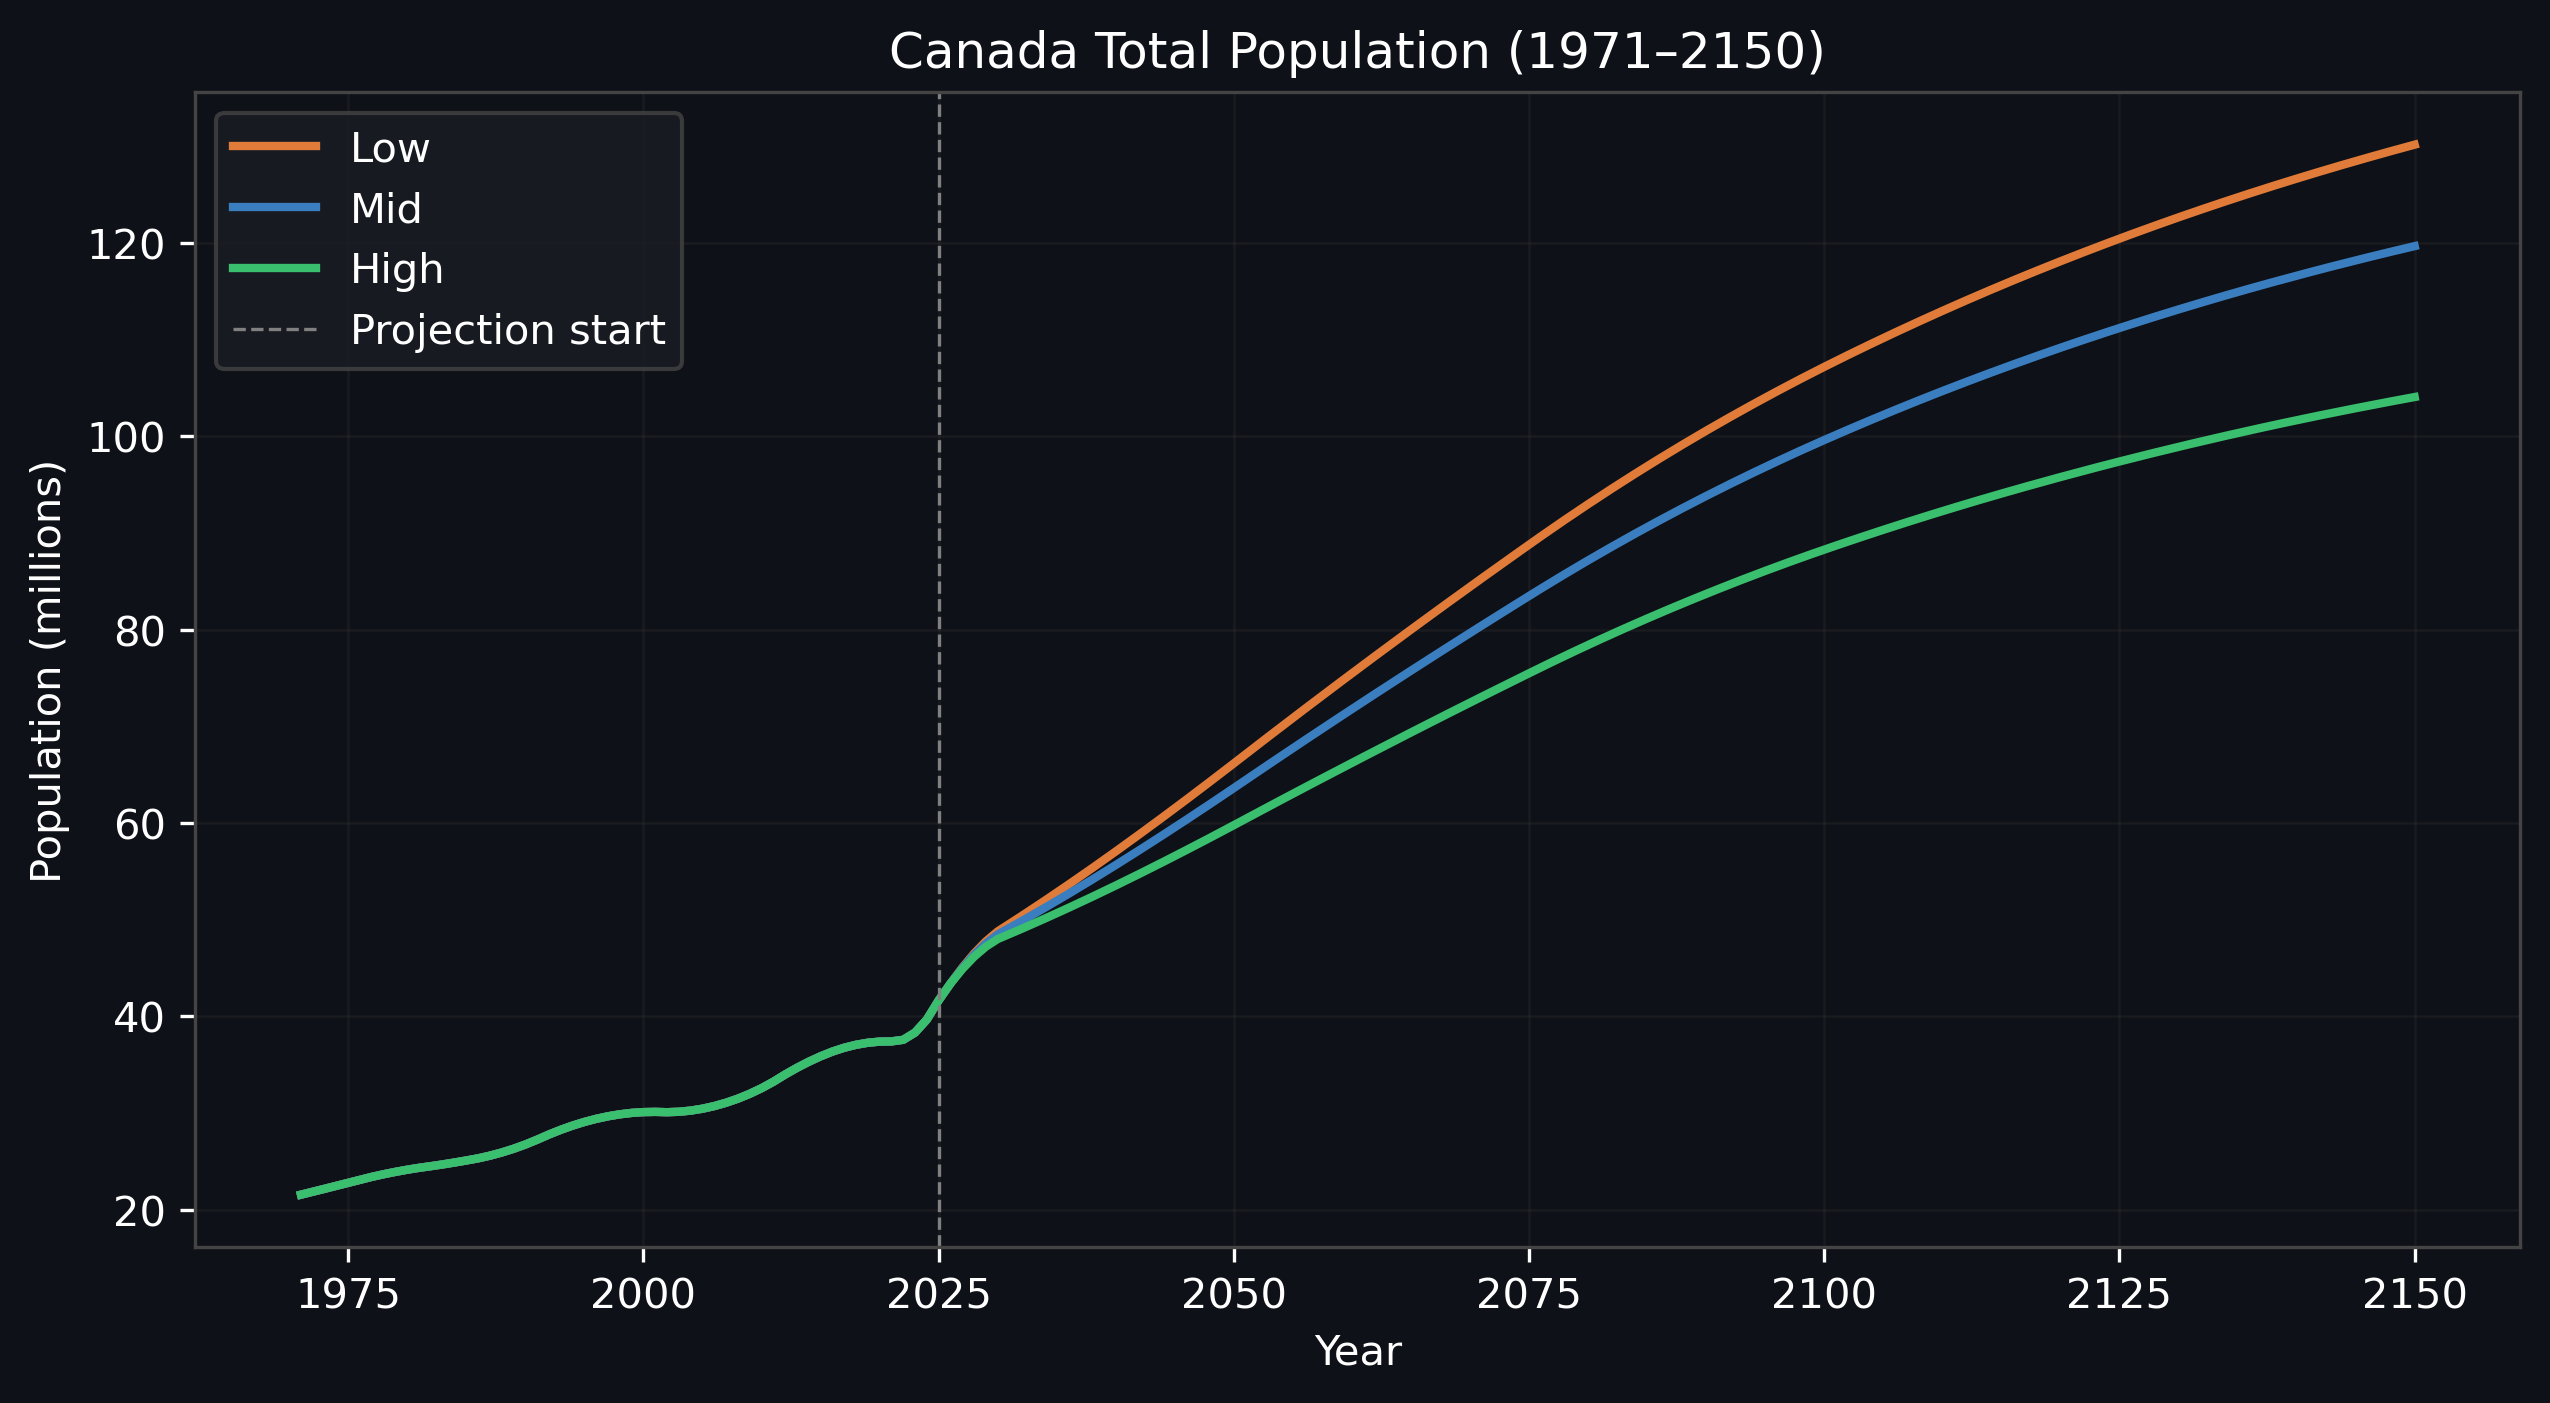
\includegraphics[width=\linewidth]{plots/01_total_population.png}
  \caption{Simulated total population of Canada by scenario (1971--2150).
           The three scenarios are identical during the 1971--2025 calibration
           period and diverge post-2025 based on different immigration volumes.
           The Mid scenario is calibrated to reach approximately 100 million
           by 2100.}
  \label{fig:total_pop}
\end{figure}

At each annual time step the model applies four processes in sequence:

\begin{enumerate}[leftmargin=1.5em]
  \item \textbf{Language transfer} --- a small fraction of agents switch
        language groups each year, using province-specific rates calibrated to
        historical census data.  In Quebec, allophones shift toward French
        (reflecting Bill 101); outside Quebec, francophones shift toward English.
  \item \textbf{Interprovincial migration} --- agents move between provinces
        using historical flow rates, with language-group multipliers reflecting
        empirical asymmetries (e.g.\ Quebec francophones are highly immobile;
        Quebec anglophones historically left at 2.5$\times$ the provincial
        average).
  \item \textbf{Natural increase} --- agents are added or removed to reflect
        net births minus deaths.  New agents inherit the language distribution
        of their province.  Most provinces are projected to have negative
        natural increase by the 2030s.
  \item \textbf{International immigration} --- new agents arrive each year,
        allocated to provinces and assigned a language based on the assumed
        composition of the immigrant intake.
\end{enumerate}

\subsection{Why the Decline Slows: The Plateau Mechanism}

A key analytical result that shapes how all the projection curves look is the
\emph{self-decelerating} nature of immigration-driven share dilution.

Each year, immigration pulls the francophone share toward the francophone
fraction of the immigrant intake.  But the size of that annual pull is
proportional to the gap between the current share and the immigrant share.
As the national francophone share falls and narrows toward the immigrant
fraction, the pull weakens --- the system automatically brakes.  This produces
the characteristic curved, plateauing shape of the projections rather than a
straight-line decline.

\begin{tcolorbox}[findingbox]
\textbf{Intuition.}  If immigrants are 14\% francophone and the population is
currently 18\% francophone, immigration delivers a 4-point downward pull each
year.  But once the share has fallen to 15\%, the pull is only 1 point.  The
closer the share gets to the immigrant fraction, the slower it moves.  The
decline decelerates continuously and the share approaches --- but never
crosses --- the immigrant fraction as a floor.
\end{tcolorbox}

\subsection{Calibration and Validation}

The period 1971--2025 uses empirical data and is identical across all three
scenarios.  The model is validated at census years (1971, 1991, 2001, 2011,
2021) against Statistics Canada figures for total population, national
francophone share, and Quebec francophone share.  The mid-scenario is
calibrated to reproduce Canada's population reaching approximately 100 million
by 2100, consistent with long-run IRCC planning assumptions.

\subsection{Scenarios}

Three scenarios govern the post-2025 projection period.  They differ on two
dimensions: the total volume of immigration and the francophone fraction of
that intake.

\begin{table}[H]
\centering
\caption{Scenario parameters applied from 2026 onward.}
\label{tab:scenarios}
\vspace{4pt}
\begin{tabular}{L{5.5cm} C{2.5cm} C{2.5cm} C{2.5cm}}
\toprule
\textbf{Parameter} & \textbf{Low} & \textbf{Mid} & \textbf{High} \\
\midrule
Immigration volume multiplier & $\times$1.10 & $\times$1.00 & $\times$0.85 \\
Francophone share offset & $-$4.0 pp & 0.0 pp & $+$4.0 pp \\
ROC francophone share (fixed) & 1.0\% & 4.0\% & 8.9\% \\
\midrule
\textit{Interpretation} & Pessimistic & Trend & Optimistic \\
\bottomrule
\end{tabular}
\end{table}

The \textbf{Low} scenario represents a pessimistic outcome for French: higher
immigration volumes combined with a reduced francophone intake share.  The
\textbf{High} scenario represents sustained federal commitment to francophone
immigration targets with moderately reduced overall volumes.  The \textbf{Mid}
scenario is a trend continuation, holding existing patterns broadly constant.


% ═════════════════════════════════════════════════════════════════════════════
\section{Data Sources}
% ═════════════════════════════════════════════════════════════════════════════

All model inputs are stored as CSV files in the \texttt{data/} directory.
Table~\ref{tab:sources} summarises the primary data sources used for each
component.

\begin{table}[H]
\centering
\caption{Primary data sources by model component.}
\label{tab:sources}
\vspace{4pt}
\begin{tabularx}{\linewidth}{L{4cm} X}
\toprule
\textbf{Component} & \textbf{Source} \\
\midrule
Initial population (1971) &
  Statistics Canada, \textit{1971 Census of Canada}.  Population by province;
  language shares from ``language spoken most often at home.'' \\
\addlinespace
Historical population benchmarks &
  Statistics Canada Census of Canada, 1971--2021 (quinquennial).
  StatCan quarterly estimate Q1 2025 ($\approx$41.5 million). \\
\addlinespace
Francophone share targets &
  Statistics Canada Census 1971--2021 --- French spoken most often at home,
  national and Quebec-specific series. \\
\addlinespace
Natural increase rates &
  Statistics Canada CANSIM Table 17-10-0008: annual births, deaths, and net
  natural increase by province, 1971--2024. \\
\addlinespace
Interprovincial migration flows &
  Statistics Canada CANSIM Table 17-10-0015: annual interprovincial migrants
  by origin and destination province. \\
\addlinespace
Language transfer rates &
  Statistics Canada \textit{Language Projections, 2011--2036}
  (Cat.\ 89-657-X) and OQLF data sheets. \\
\addlinespace
Immigration volume (1971--2025) &
  IRCC annual permanent resident landings data and the 2025 immigration
  levels plan. \\
\addlinespace
Immigrant francophone share --- Quebec &
  Office qu\'{e}b\'{e}cois de la langue fran\c{c}aise (OQLF) and
  Minist\`{e}re de l'Immigration, de la Francisation et de l'Int\'{e}gration
  (MIFI), 2001--2025. \\
\addlinespace
Immigrant francophone share --- ROC &
  IRCC Annual Reports 2003--2025 (federal francophone immigration target
  data and achievement rates). \\
\bottomrule
\end{tabularx}
\end{table}

Post-2025 values in all input files are projections based on trend
extrapolation of the above sources.  They do not represent official Statistics
Canada or Government of Canada forecasts.


% ═════════════════════════════════════════════════════════════════════════════
\section{Model Parameters}
% ═════════════════════════════════════════════════════════════════════════════

\subsection{Starting Population --- 1971 Census}

The simulation is initialised from the 1971 Census.  Table~\ref{tab:init_pop}
shows the starting population and language composition for each province.
Quebec is the only province with a francophone majority.  New Brunswick at
31\% is the only other province with a substantial francophone share.

\begin{table}[H]
\centering
\caption{Initial population and language shares by province, 1971 Census.}
\label{tab:init_pop}
\vspace{4pt}
\begin{tabular}{L{2.5cm} R{2.4cm} R{2.2cm} R{2.2cm} R{2.2cm}}
\toprule
\textbf{Province} & \textbf{Population} & \textbf{Fr share} & \textbf{En share} & \textbf{Allo share} \\
\midrule
NL & 522{,}000 & 0.3\% & 99.2\% & 0.5\% \\
PE & 112{,}000 & 4.0\% & 95.0\% & 1.0\% \\
NS & 789{,}000 & 2.5\% & 95.5\% & 2.0\% \\
NB & 635{,}000 & 31.0\% & 68.0\% & 1.0\% \\
QC & 6{,}028{,}000 & 80.8\% & 13.2\% & 6.0\% \\
ON & 7{,}703{,}000 & 4.6\% & 75.4\% & 12.0\% \\
MB & 988{,}000 & 4.5\% & 85.5\% & 11.0\% \\
SK & 926{,}000 & 1.8\% & 91.2\% & 7.0\% \\
AB & 1{,}628{,}000 & 1.4\% & 90.6\% & 8.0\% \\
BC & 2{,}185{,}000 & 0.8\% & 89.2\% & 10.0\% \\
YT, NT, NU & 53{,}000 & mixed & --- & --- \\
\midrule
\textbf{Canada} & \textbf{21{,}569{,}000} & \textbf{25.7\%} & \textbf{66.5\%} & \textbf{7.8\%} \\
\bottomrule
\end{tabular}
\end{table}

\subsection{Immigration Volume}

Annual immigrant landings follow historical IRCC data from 1971 to 2025.
After 2025 the volume is projected under each scenario.  The base trajectory
(Mid scenario multiplier = 1.0) is shown in Table~\ref{tab:imm_volume} at
selected years.

\begin{table}[H]
\centering
\caption{Annual immigration volume (base trajectory, mid scenario) at selected years.}
\label{tab:imm_volume}
\vspace{4pt}
\begin{tabular}{R{2cm} R{3cm} R{1.5cm} R{2cm} R{3cm}}
\toprule
\textbf{Year} & \textbf{Landings} & & \textbf{Year} & \textbf{Landings} \\
\midrule
1971 & 122{,}000 & & 2025 & 500{,}000 \\
1985 & 84{,}000  & & 2030 & 700{,}000 \\
2000 & 227{,}000 & & 2050 & 910{,}000 \\
2020 & 184{,}000 & & 2100 & 960{,}000 \\
2023 & 471{,}000 & & 2150 & 900{,}000 \\
\bottomrule
\end{tabular}
\end{table}

The 2020 dip reflects COVID-19 border restrictions.  The post-2030 ramp
reflects continuation of the trajectory set by IRCC's 2025 levels plan,
scaled to meet the 100-million-by-2100 calibration target in the Mid scenario.

\subsection{Linguistic Composition of Immigrants}

Quebec and the Rest of Canada operate under different selection regimes,
producing very different linguistic profiles in the immigrant intake.

\begin{table}[H]
\centering
\caption{Francophone share of immigrants by destination region at selected years
         (mid scenario). Post-2025 values are trend projections; scenario offsets
         and overrides are applied on top.}
\label{tab:imm_comp}
\vspace{4pt}
\begin{tabular}{R{1.5cm} R{3.5cm} R{3.5cm}}
\toprule
\textbf{Year} & \textbf{Quebec fr share} & \textbf{ROC fr share} \\
\midrule
1971 & 35.0\% & 2.0\% \\
2001 & 51.0\% & 3.0\% \\
2016 & 60.5\% (peak) & 3.0\% \\
2021 & 54.5\% & 4.5\% \\
2025 & 56.0\% & 8.9\% \\
2050 & 49.0\% & 8.2\% \\
2100 & 41.5\% & 7.5\% \\
2150 & 39.0\% & 7.0\% \\
\bottomrule
\end{tabular}
\end{table}

The Quebec series peaked in 2016 (60.5\% per OQLF data), driven by Bill 101
enforcement and active Quebec selection of French-speaking immigrants.  The
subsequent decline reflects structural shifts in source-country composition.
The ROC series rose sharply from 2022--2025 on a surge of francophone
Sub-Saharan African arrivals, then stabilises below the federal government's
aspirational 12\% target.

\subsection{Language Transfer Rates}

Every year a small fraction of agents shift language groups, reflecting
intergenerational assimilation.  Table~\ref{tab:lt} shows the most
policy-relevant rates calibrated to the 2021 period.

\begin{table}[H]
\centering
\caption{Annual language transfer rates at the 2021 calibration point.
         These are per-person annual probabilities of switching language group.}
\label{tab:lt}
\vspace{4pt}
\begin{tabular}{L{2cm} L{1.5cm} L{1.5cm} C{2.5cm} L{5.5cm}}
\toprule
\textbf{Region} & \textbf{From} & \textbf{To} & \textbf{Annual rate} & \textbf{Context} \\
\midrule
Quebec & Allo & French & 1.6\% / yr & Bill 101 French integration \\
Quebec & Allo & English & 1.0\% / yr & Declining English pull \\
Quebec & English & French & 0.25\% / yr & Modest Anglo-to-French shift \\
Quebec & French & English & 0.05\% / yr & Negligible \\
\addlinespace
NB & French & English & 0.6\% / yr & Gradual Acadian erosion \\
\addlinespace
ROC & French & English & 1.8\% / yr & $\approx$41\% cumulative lifetime \\
ROC & Allo & English & 2.0\% / yr & $\approx$50\% cumulative lifetime \\
ROC & Allo & French & 0.06\% / yr & Minimal francophone retention \\
\bottomrule
\end{tabular}
\end{table}

The ROC francophone-to-English rate of 1.8\% per year is the highest of any
group and reflects the assimilation pressure faced by small francophone
communities embedded in overwhelmingly anglophone environments.

\subsection{Interprovincial Migration and Language Multipliers}

Base migration flows are calibrated from StatCan data for three anchor periods
(1971, 2000, 2024).  Table~\ref{tab:lang_mult} shows the language-specific
multipliers that adjust the base out-migration rate for particular
province-language combinations.

\begin{table}[H]
\centering
\caption{Language-conditional out-migration multipliers (1.0 = provincial average).}
\label{tab:lang_mult}
\vspace{4pt}
\begin{tabular}{L{2.5cm} L{2.5cm} C{2.5cm} L{5cm}}
\toprule
\textbf{Province} & \textbf{Language} & \textbf{Multiplier} & \textbf{Reason} \\
\midrule
Quebec & Francophone & 0.30 & Francophone Quebecers are highly immobile \\
Quebec & Anglophone  & 2.50 & Post-1976 Anglo exodus \\
Quebec & Allophone   & 1.50 & Above-average departure \\
Ontario & Francophone & 1.50 & Franco-Ontarians above-average mobile \\
NB      & Francophone & 0.70 & Acadian community stickiness \\
Manitoba & Francophone & 1.30 & Small community, mobile \\
Alberta  & Francophone & 2.00 & Oil-sector high mobility \\
BC       & Francophone & 1.80 & Small dispersed community \\
\bottomrule
\end{tabular}
\end{table}


% ═════════════════════════════════════════════════════════════════════════════
\section{Key Findings}
% ═════════════════════════════════════════════════════════════════════════════

\subsection{Finding 1 --- National Francophone Share Declines but Plateaus}

Under all three scenarios, Canada's national francophone share falls
continuously from approximately 19\% in 2025 (Figure~\ref{fig:national_share}).
By 2150 the share reaches 8\% under the Low scenario, 9.5\% under Mid, and
12\% under High.  The High scenario visibly flattens after 2100, approaching
its equilibrium.  Under Low, the decline continues more steeply throughout,
reflecting the compounding of higher volume and lower francophone intake share.

\begin{figure}[H]
  \centering
  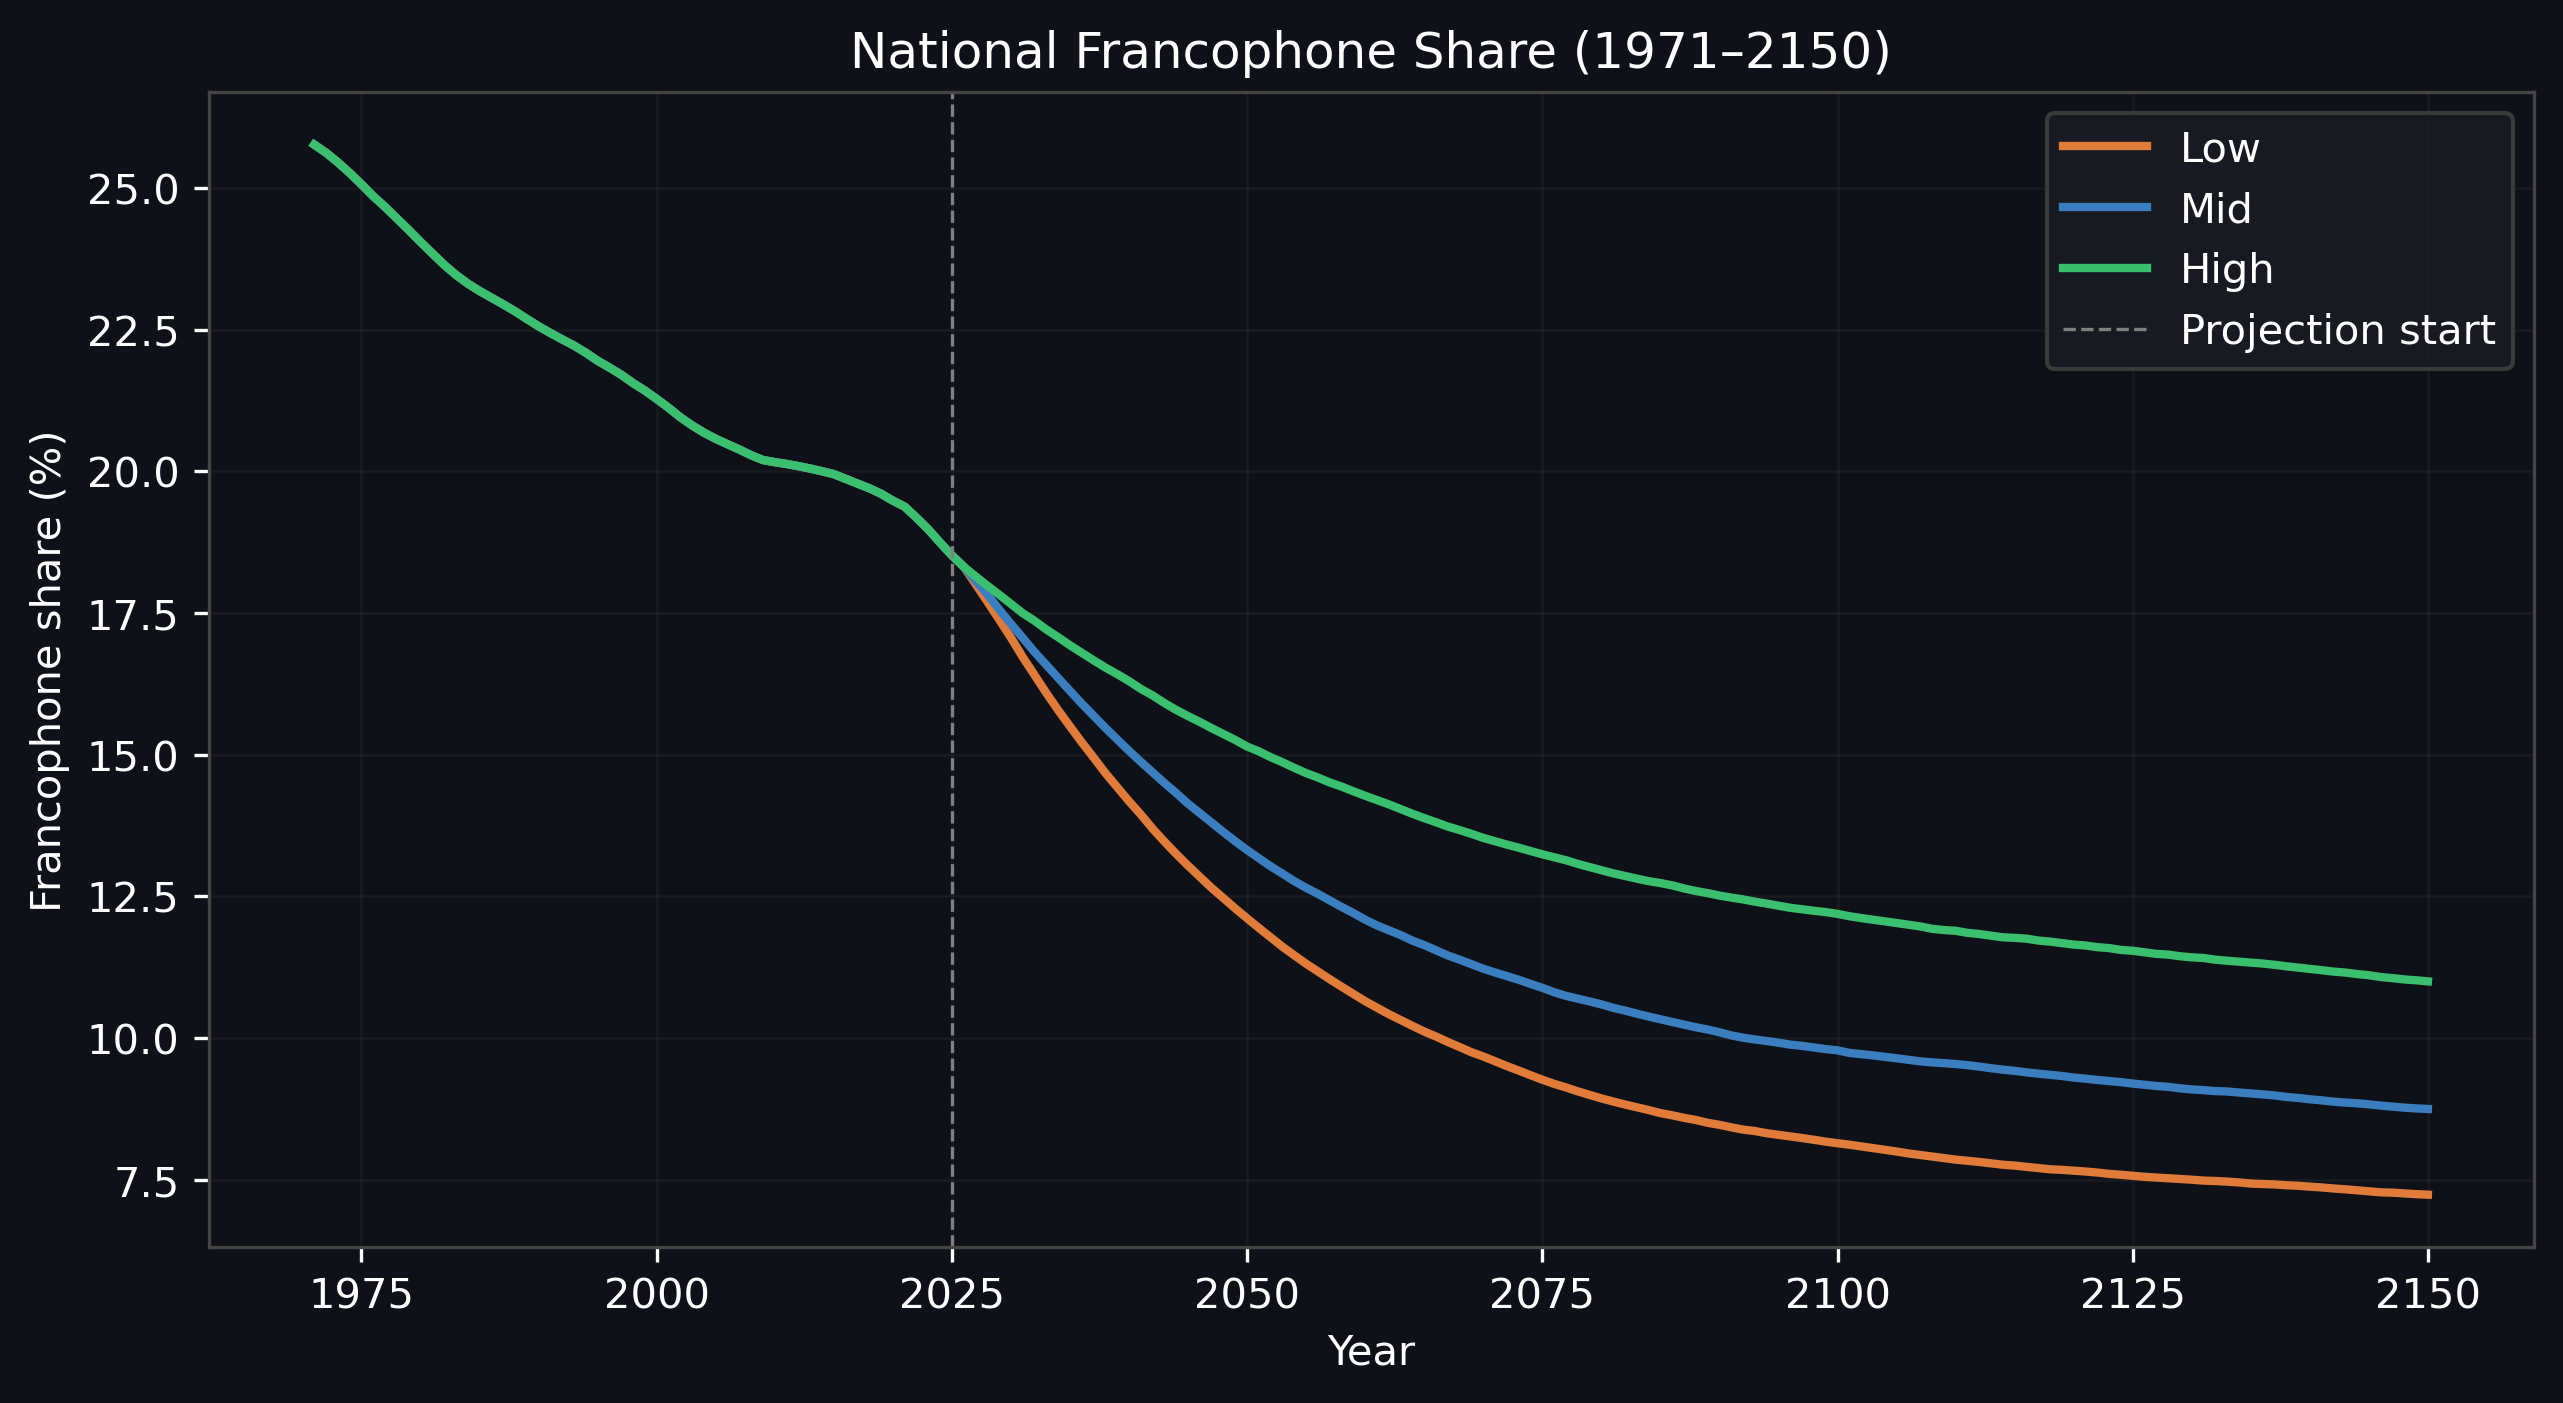
\includegraphics[width=\linewidth]{plots/02_national_fr_share.png}
  \caption{National francophone share of Canada's total population (1971--2150)
           under three scenarios.  The dashed vertical line marks the end of
           the calibration period.  All three scenarios reproduce the
           historical 1971--2025 decline and diverge thereafter.}
  \label{fig:national_share}
\end{figure}

The curves are visibly curved rather than straight.  This is the plateau
mechanism described in Section 1.2: each year's dilution force is proportional
to the gap between the current share and the immigrant share, so as the share
falls, the force weakens.

\begin{tcolorbox}[findingbox]
\textbf{Key takeaway.}  The national francophone share will roughly halve
from its 2025 level by 2150 in the Mid scenario.  The difference between
Low and High by 2150 is approximately 4 percentage points --- a meaningful
but bounded range of outcomes.
\end{tcolorbox}

\subsection{Finding 2 --- The Dilution Gap Narrows Toward Equilibrium}

Figure~\ref{fig:overlay} overlays the national francophone share $f(t)$
(solid lines) with the effective francophone fraction of immigrants
$f_{\text{imm}}$ (dashed lines) for each scenario.  The gap between solid and
dashed is the engine driving the decline each year.

\begin{figure}[H]
  \centering
  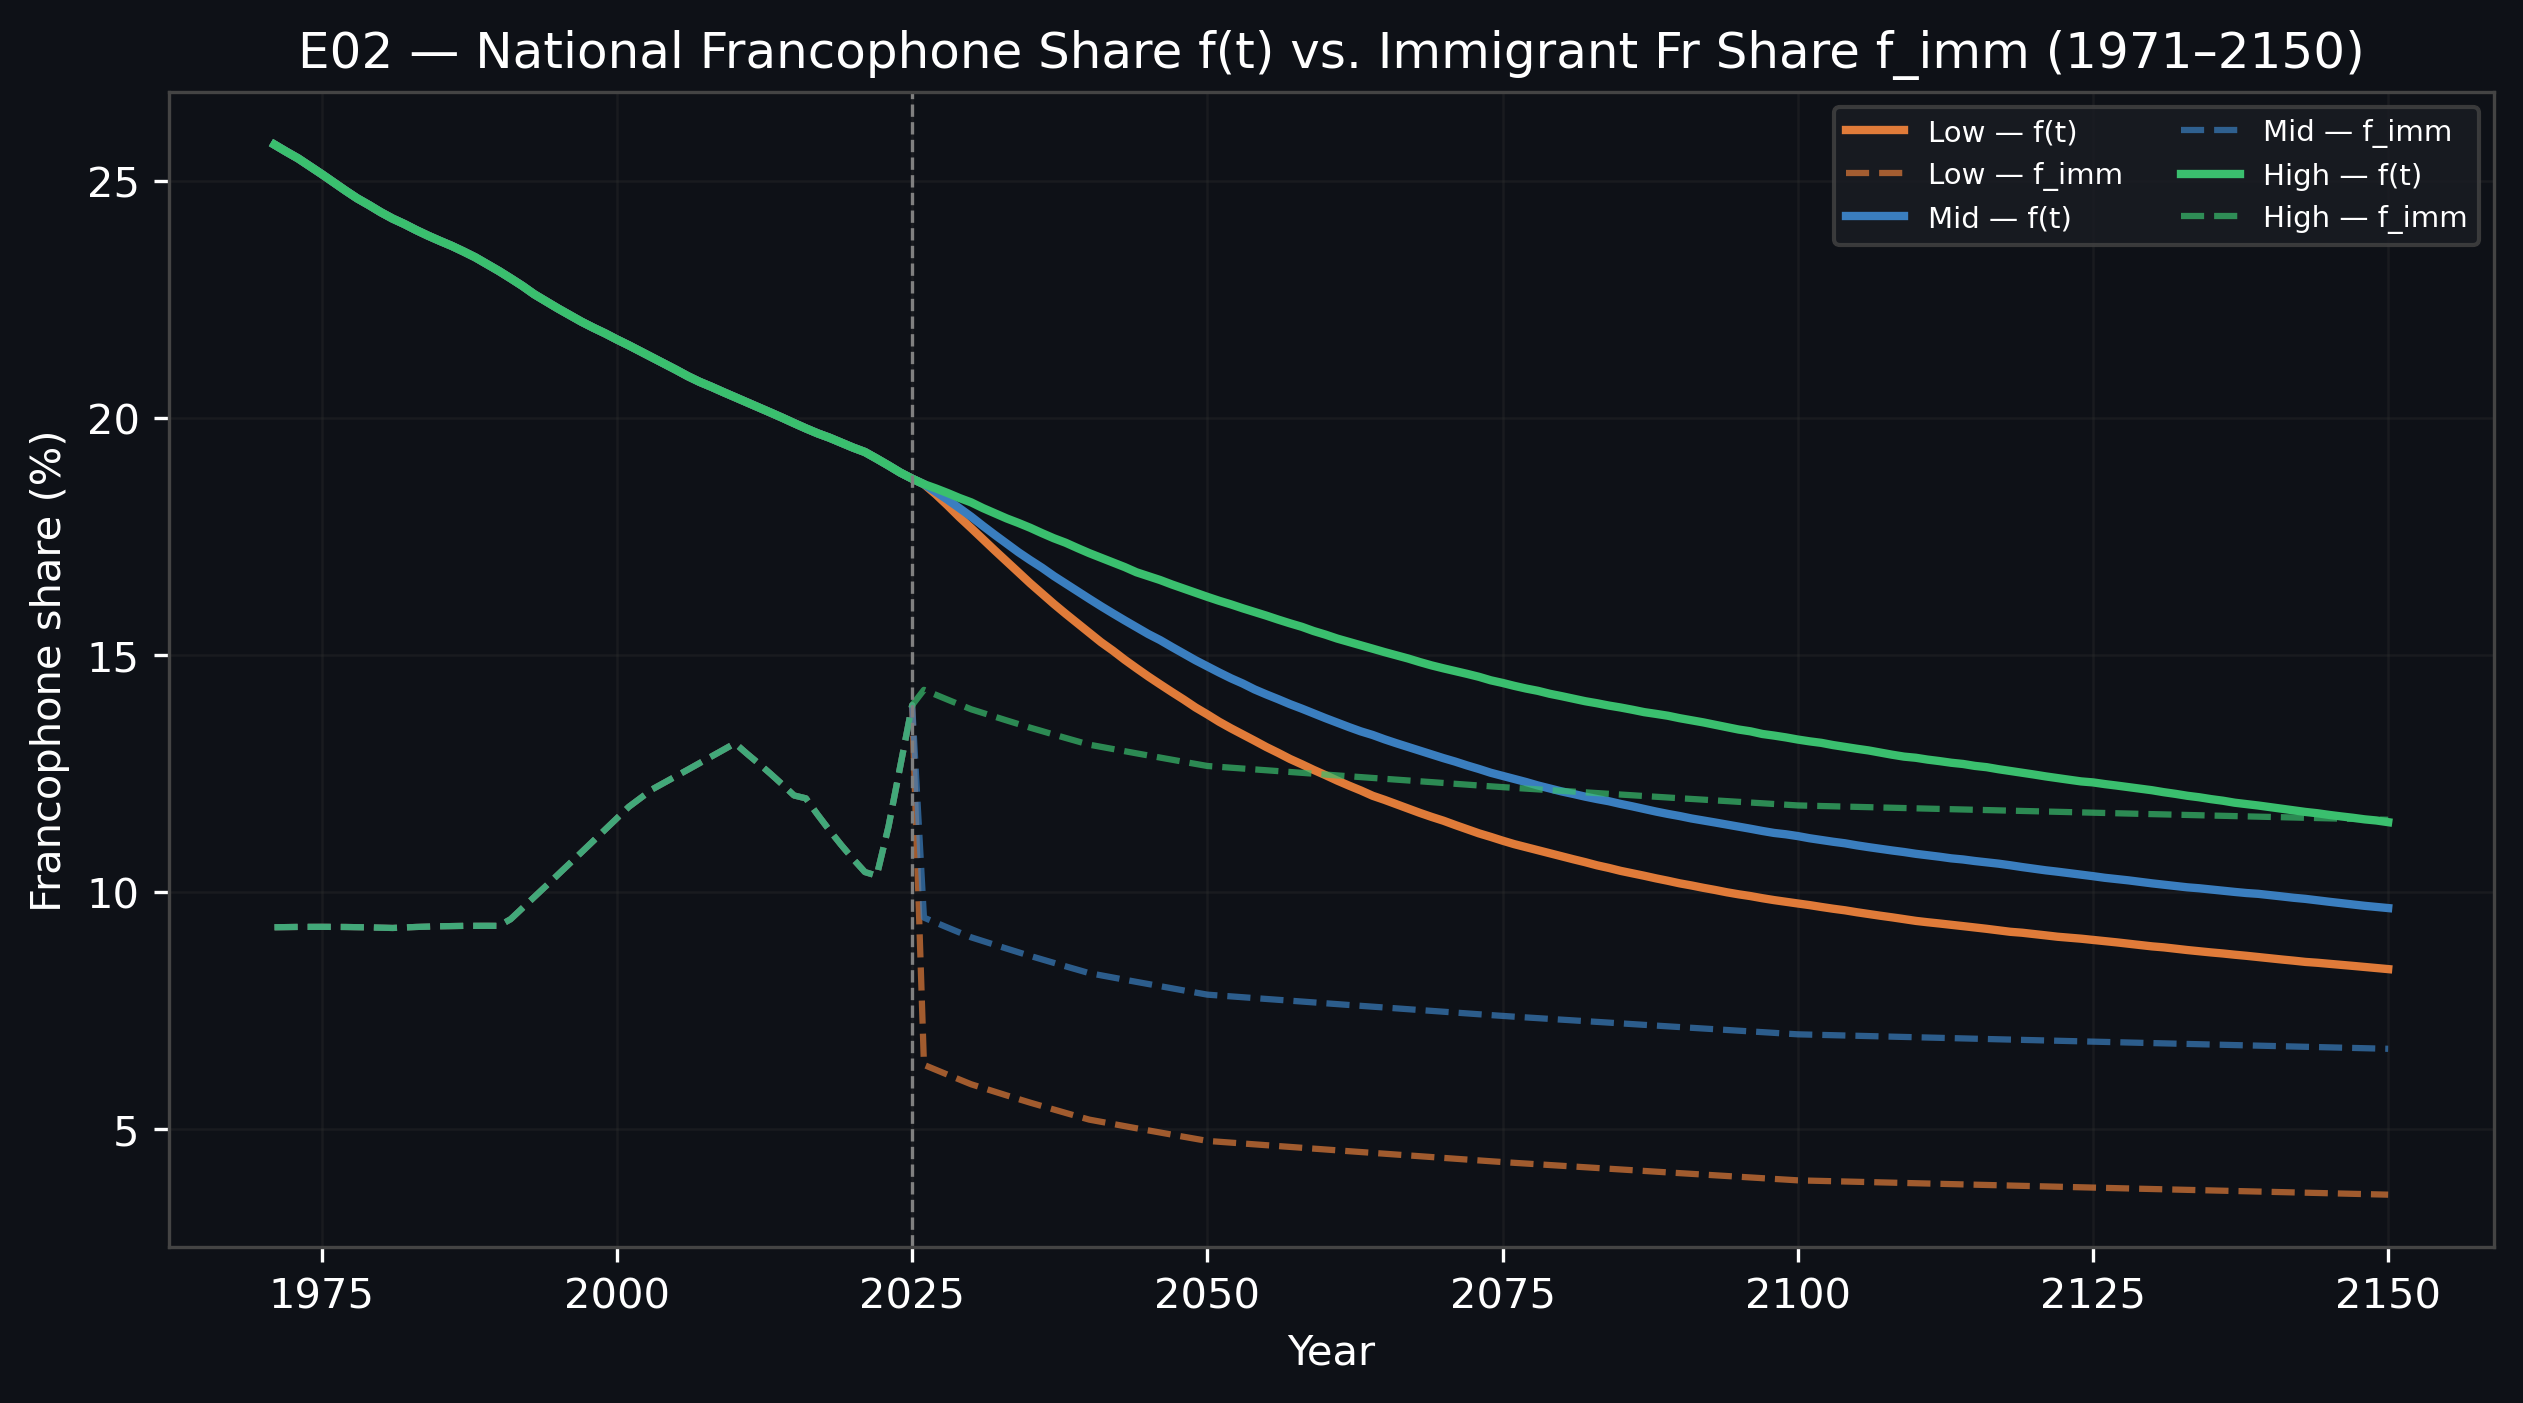
\includegraphics[width=\linewidth]{plots/E02_ft_vs_fimm_overlay.png}
  \caption{National francophone share $f(t)$ (solid) vs.\ effective francophone
           share of annual immigrants $f_{\text{imm}}$ (dashed) by scenario.
           The solid lines chase the dashed lines from above; the gap between
           them drives the rate of decline.}
  \label{fig:overlay}
\end{figure}

The sharp drop in the dashed lines at 2025 reflects the scenario offsets
taking effect.  In the Low scenario, the immigrant francophone share is
effectively just 6\% after 2025 --- far below the population share ---
explaining the steep initial decline.  In the High scenario, $f_{\text{imm}}$
is held near 12--14\%, and the solid line approaches it slowly, producing the
visible plateau after 2100.

\subsection{Finding 3 --- Francophones Grow in Absolute Numbers}

Figure~\ref{fig:abs_fr} shows that despite declining in share, the francophone
population grows in absolute terms throughout the projection period under all
scenarios.

\begin{figure}[H]
  \centering
  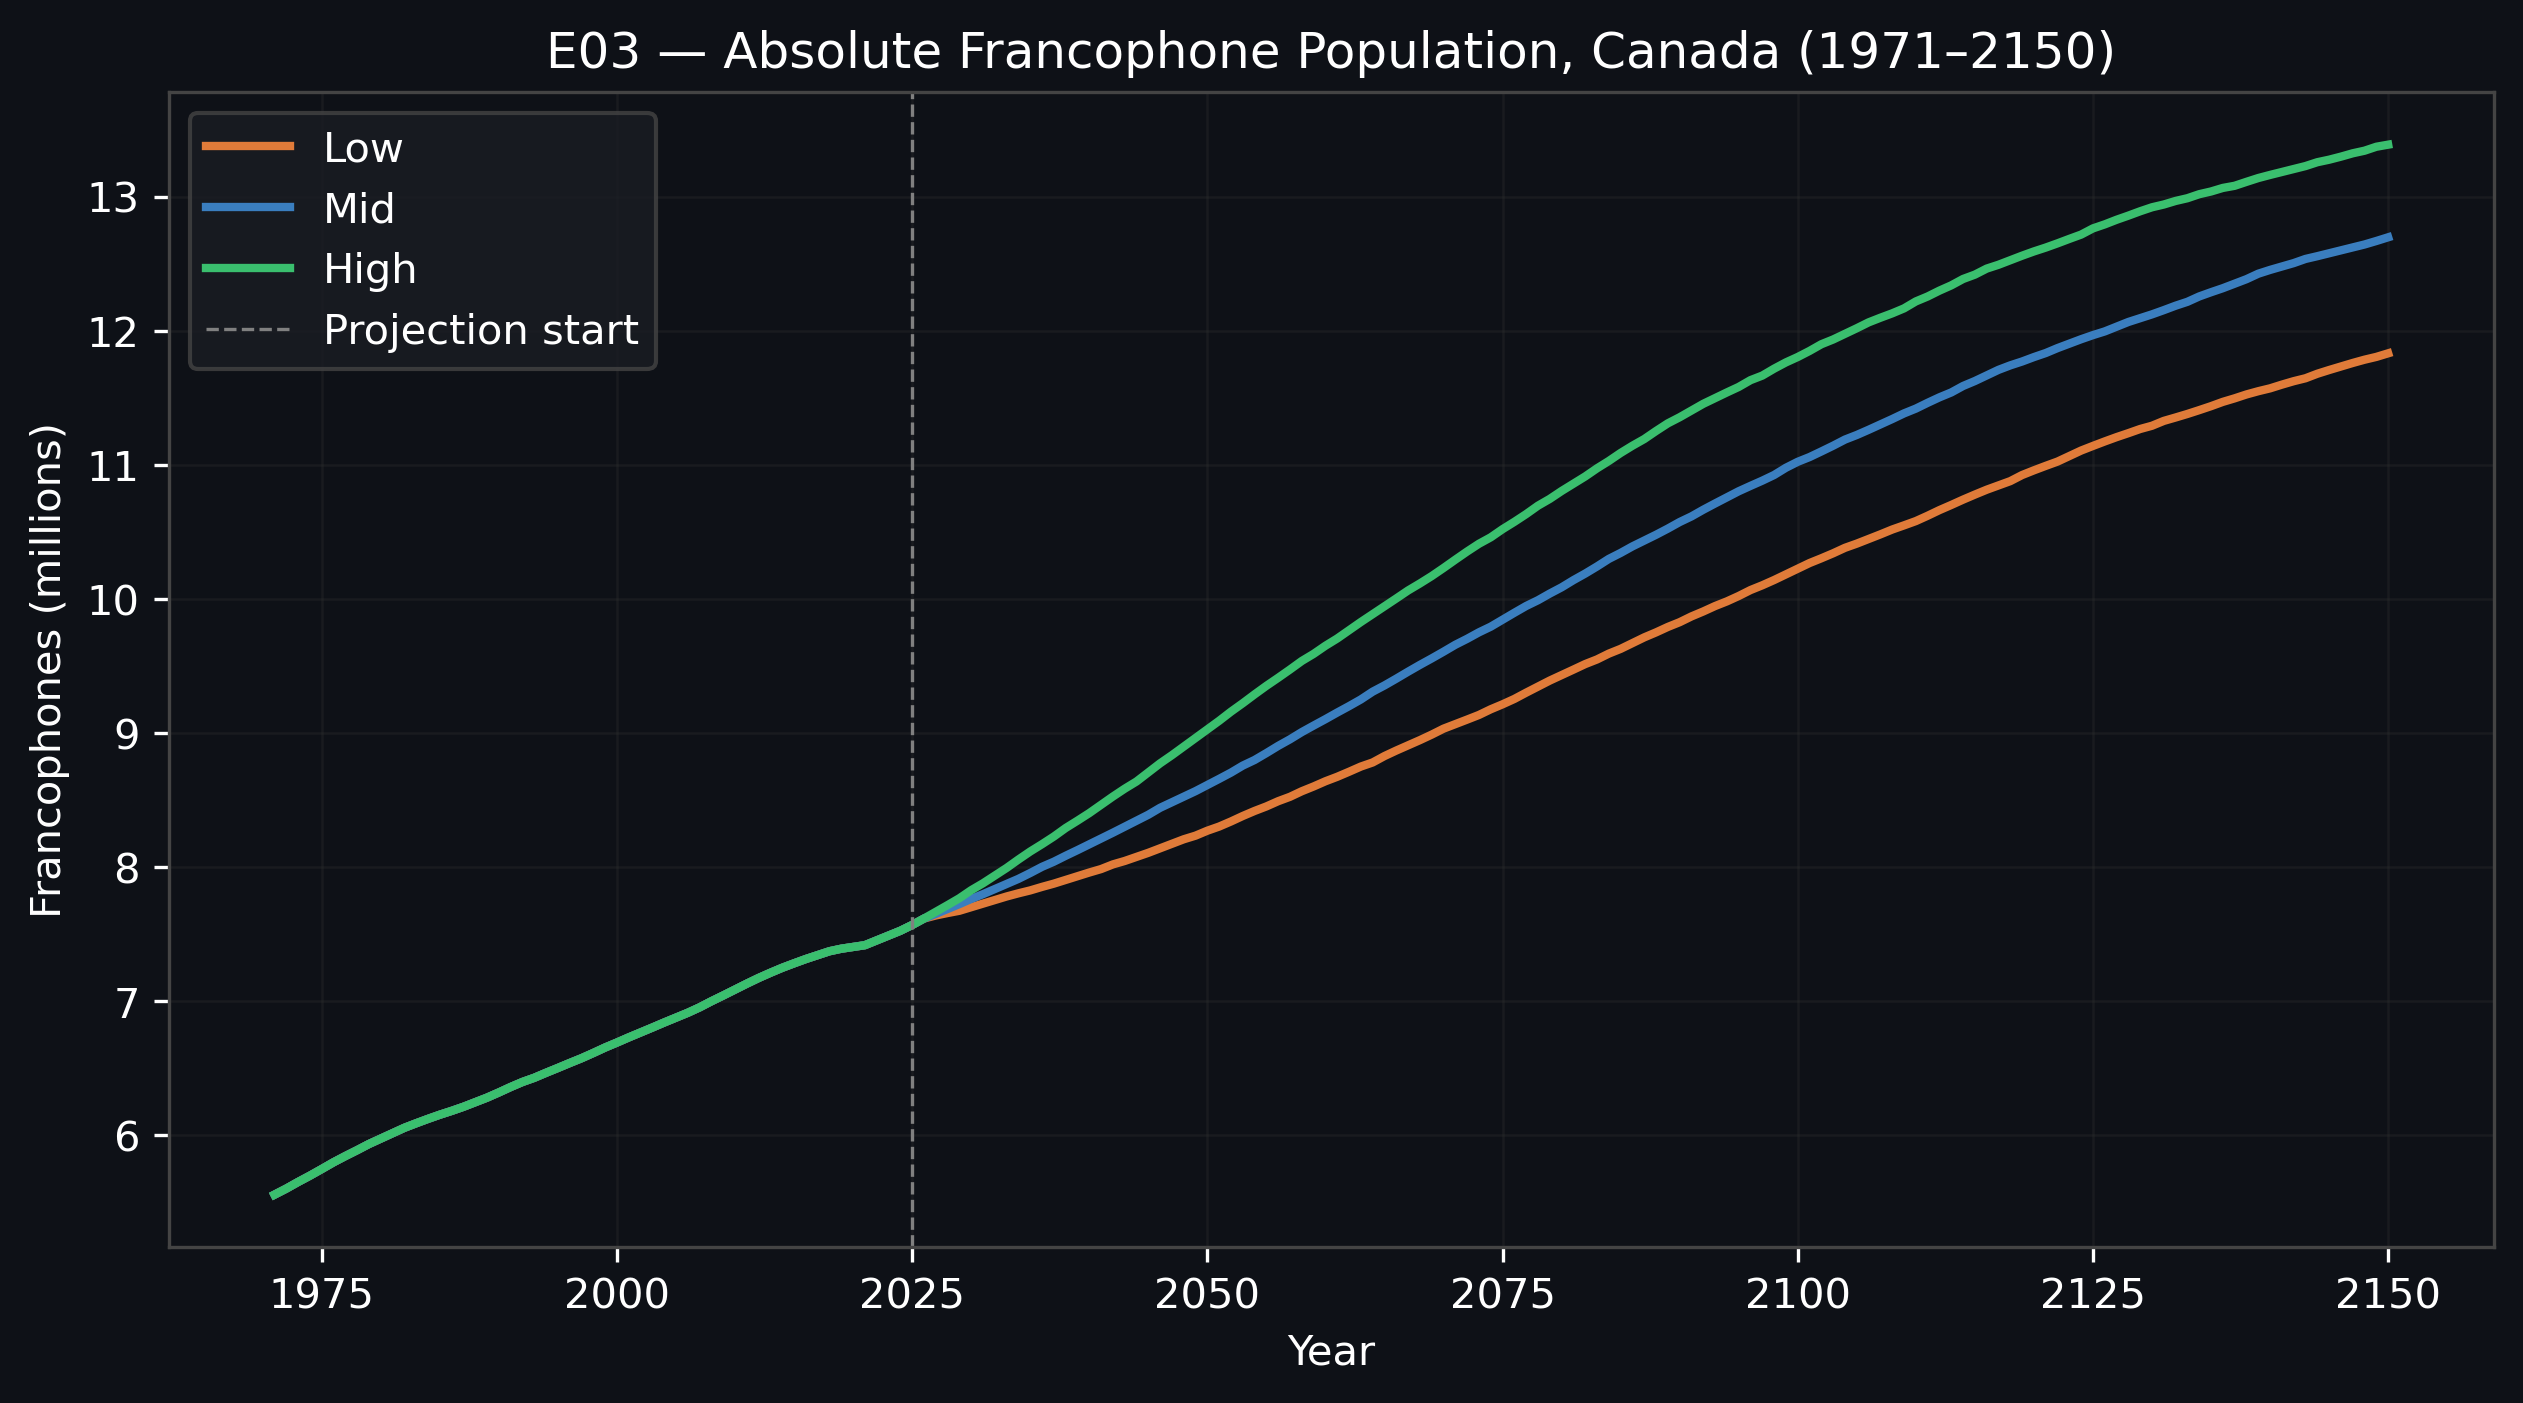
\includegraphics[width=\linewidth]{plots/E03_absolute_francophone_pop.png}
  \caption{Total francophone population of Canada in millions (1971--2150).
           All three scenarios show continuous growth, reflecting the large
           base population and continued francophone immigration.}
  \label{fig:abs_fr}
\end{figure}

\begin{tcolorbox}[statbox]
The francophone population grows from \textbf{7.5 million} in 2025 to
\textbf{12--13 million} by 2150.  The share decline is almost entirely a
denominator effect: non-francophone Canadians grow considerably faster, not
because there are fewer francophones, but because there are substantially more
of everyone else.
\end{tcolorbox}

This distinction is important for policy.  Institutions serving francophone
Canadians will face a \emph{larger} absolute population even as that
population represents a declining fraction of the total.  The policy challenge
is not protecting a shrinking community but maintaining relative influence and
institutional capacity for a growing one.

\subsection{Finding 4 --- Quebec Holds; the Rest of Canada Does Not}

Figures~\ref{fig:qc_share} and~\ref{fig:roc_share} show the divergence between
Quebec and the Rest of Canada --- the simulation's most consequential regional
split.

\begin{figure}[H]
  \centering
  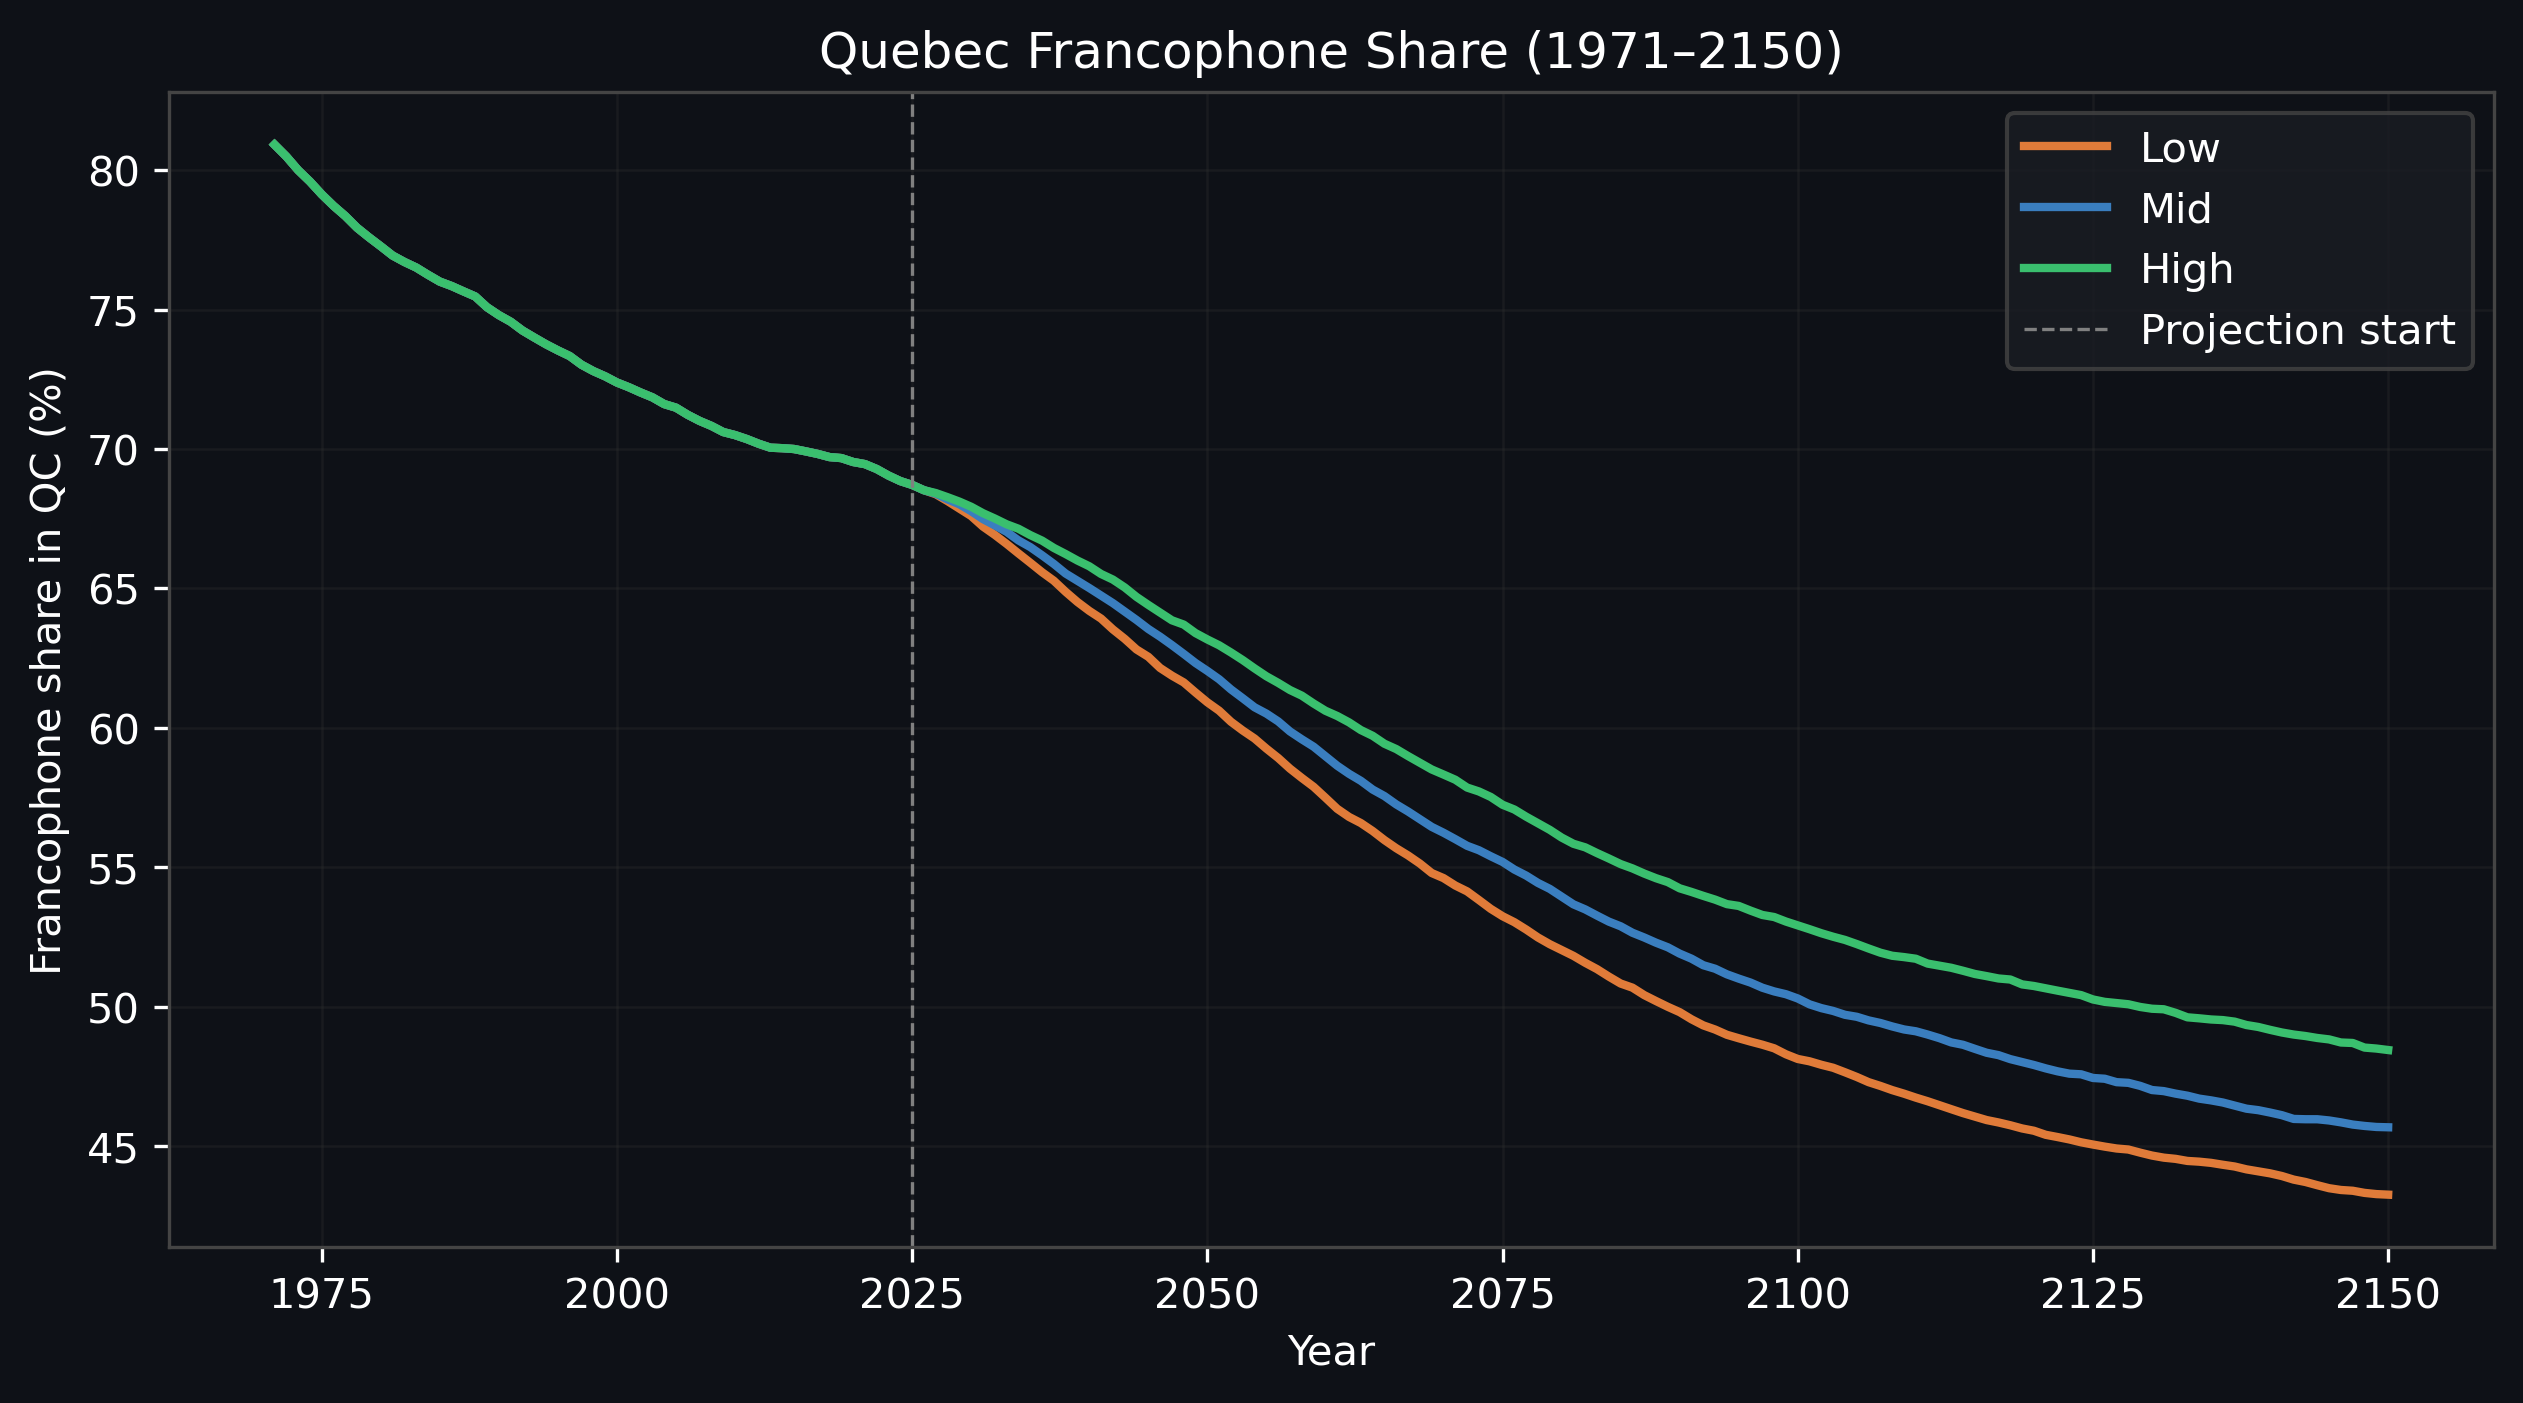
\includegraphics[width=\linewidth]{plots/03_qc_fr_share.png}
  \caption{Quebec's internal francophone share (1971--2150).  All scenarios
           project Quebec remaining above 70\% francophone throughout, with
           a slow decline driven by growing allophone immigration.}
  \label{fig:qc_share}
\end{figure}

Quebec's francophone share declines modestly but remains dominant across all
scenarios.  It falls from 77.5\% in 2021 to approximately 65--72\% by 2150,
depending on scenario.  Bill 101 continues to drive allophone integration into
French, and Quebec's own selection process sustains a majority francophone
immigrant intake.

\begin{figure}[H]
  \centering
  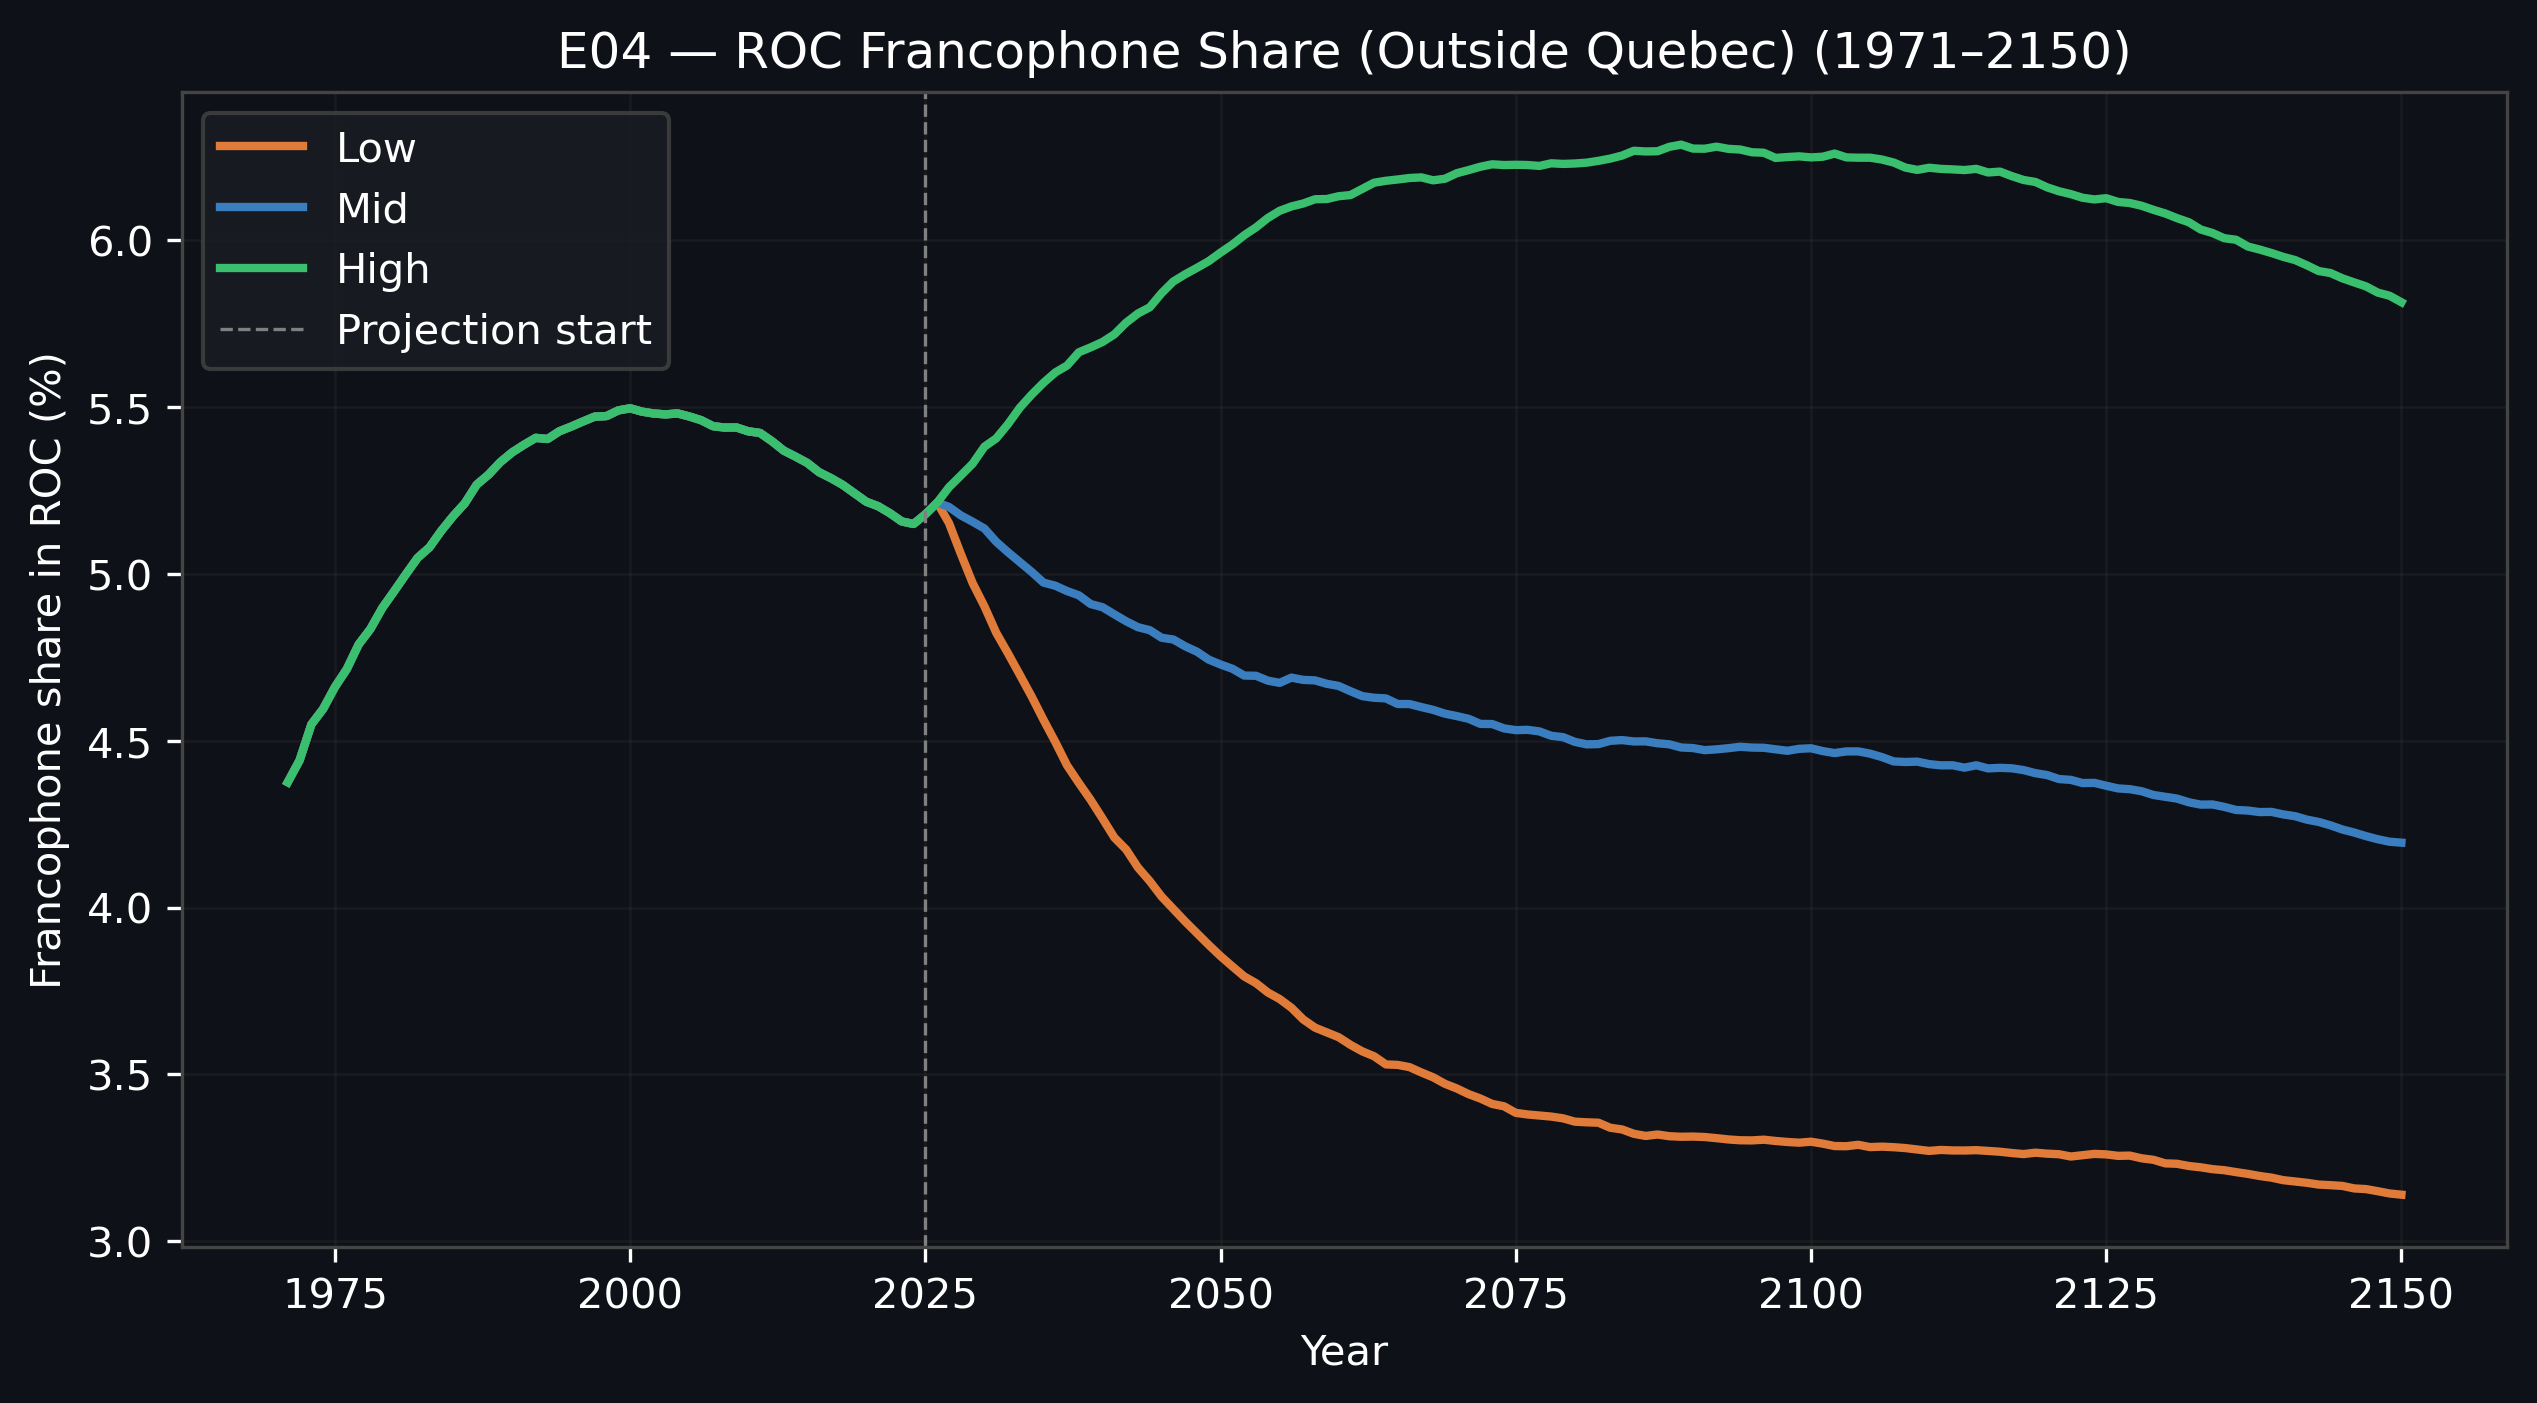
\includegraphics[width=\linewidth]{plots/E04_roc_fr_share.png}
  \caption{Francophone share of the Rest of Canada (outside Quebec), 1971--2150.
           The decline is considerably steeper than the national aggregate,
           driven by low francophone immigration shares and high
           French-to-English language transfer.}
  \label{fig:roc_share}
\end{figure}

Outside Quebec, the picture is starkly different.  The ROC francophone share
falls from approximately 5.3\% in 2025 to between 3.0\% (Low) and 4.2\% (Mid)
by 2150.  Only the High scenario --- with its elevated ROC francophone
immigration override --- bucks the trend, rising briefly to 6.3\% before
declining.

The ROC decline is driven by two forces simultaneously: the same
immigration-driven dilution present nationally, but with a far lower
francophone intake fraction; and a language transfer rate from French to
English ($\approx$1.8\%/year) that is almost 36 times higher than the
equivalent rate in Quebec.

\begin{tcolorbox}[findingbox]
\textbf{Key takeaway.}  Quebec's francophone majority is robust across all
scenarios.  The existential question for French in Canada is not Quebec ---
it is the survival of francophone communities outside it.  ROC francophones
are under pressure from both dilution and assimilation simultaneously.
\end{tcolorbox}

\subsection{Finding 5 --- New Brunswick: Slow but Steady Erosion}

New Brunswick is Canada's only officially bilingual province and home to the
Acadian community, the largest francophone population outside Quebec.
Figure~\ref{fig:nb} tracks NB language shares under all three scenarios.

\begin{figure}[H]
  \centering
  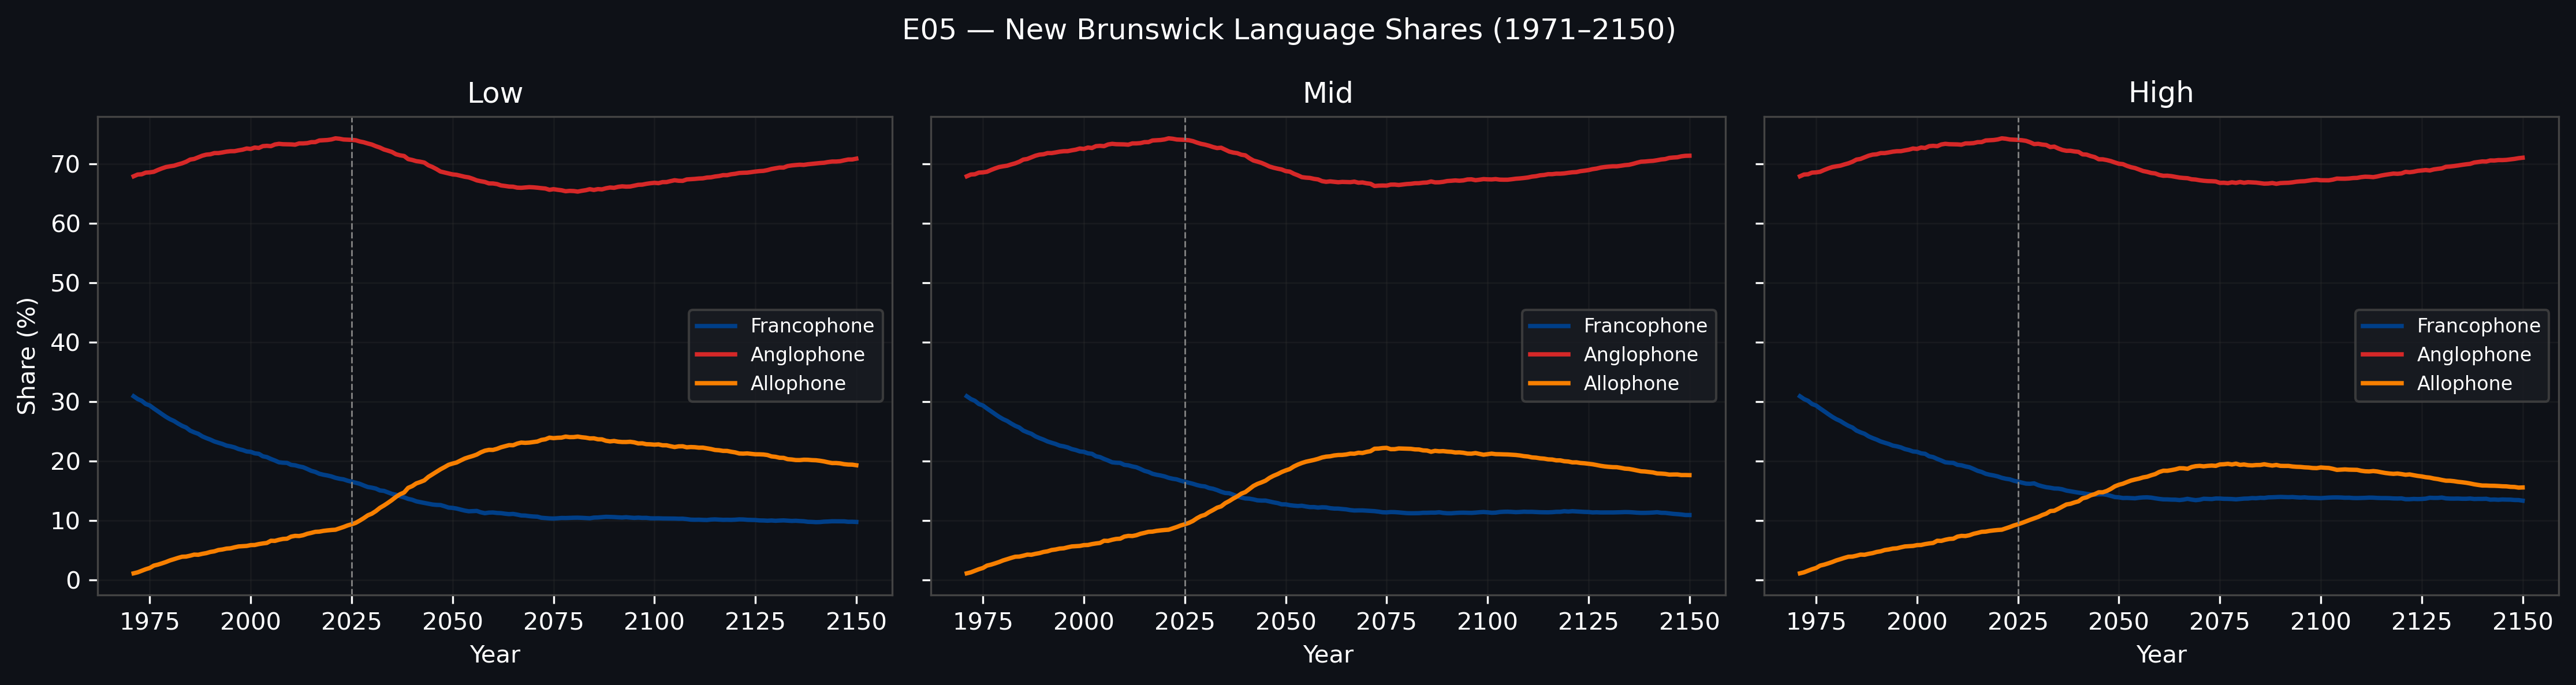
\includegraphics[width=\linewidth]{plots/E05_nb_language_shares.png}
  \caption{New Brunswick language shares under Low (left), Mid (centre), and
           High (right) scenarios.  The francophone share (blue) declines
           steadily while the allophone share (orange) grows substantially
           from near zero.}
  \label{fig:nb}
\end{figure}

The NB francophone share falls from 31\% in 1971 to between 14\% and 16\% by
2150 --- roughly halved.  Anglophones remain the dominant group but also lose
relative ground as allophones grow.  The Acadian community's below-average
out-migration rate (multiplier 0.70) and the province's bilingual institutions
provide some protection, but the erosion is sustained across all scenarios.

\subsection{Finding 6 --- Immigration Dilution Drives the Decline; Language
Transfer Is Secondary}

Figure~\ref{fig:decomp} decomposes the annual change in the national
francophone share into two components for the Mid scenario:
(1)~the immigration dilution effect and (2)~the combined effect of language
transfer and natural increase.

\begin{figure}[H]
  \centering
  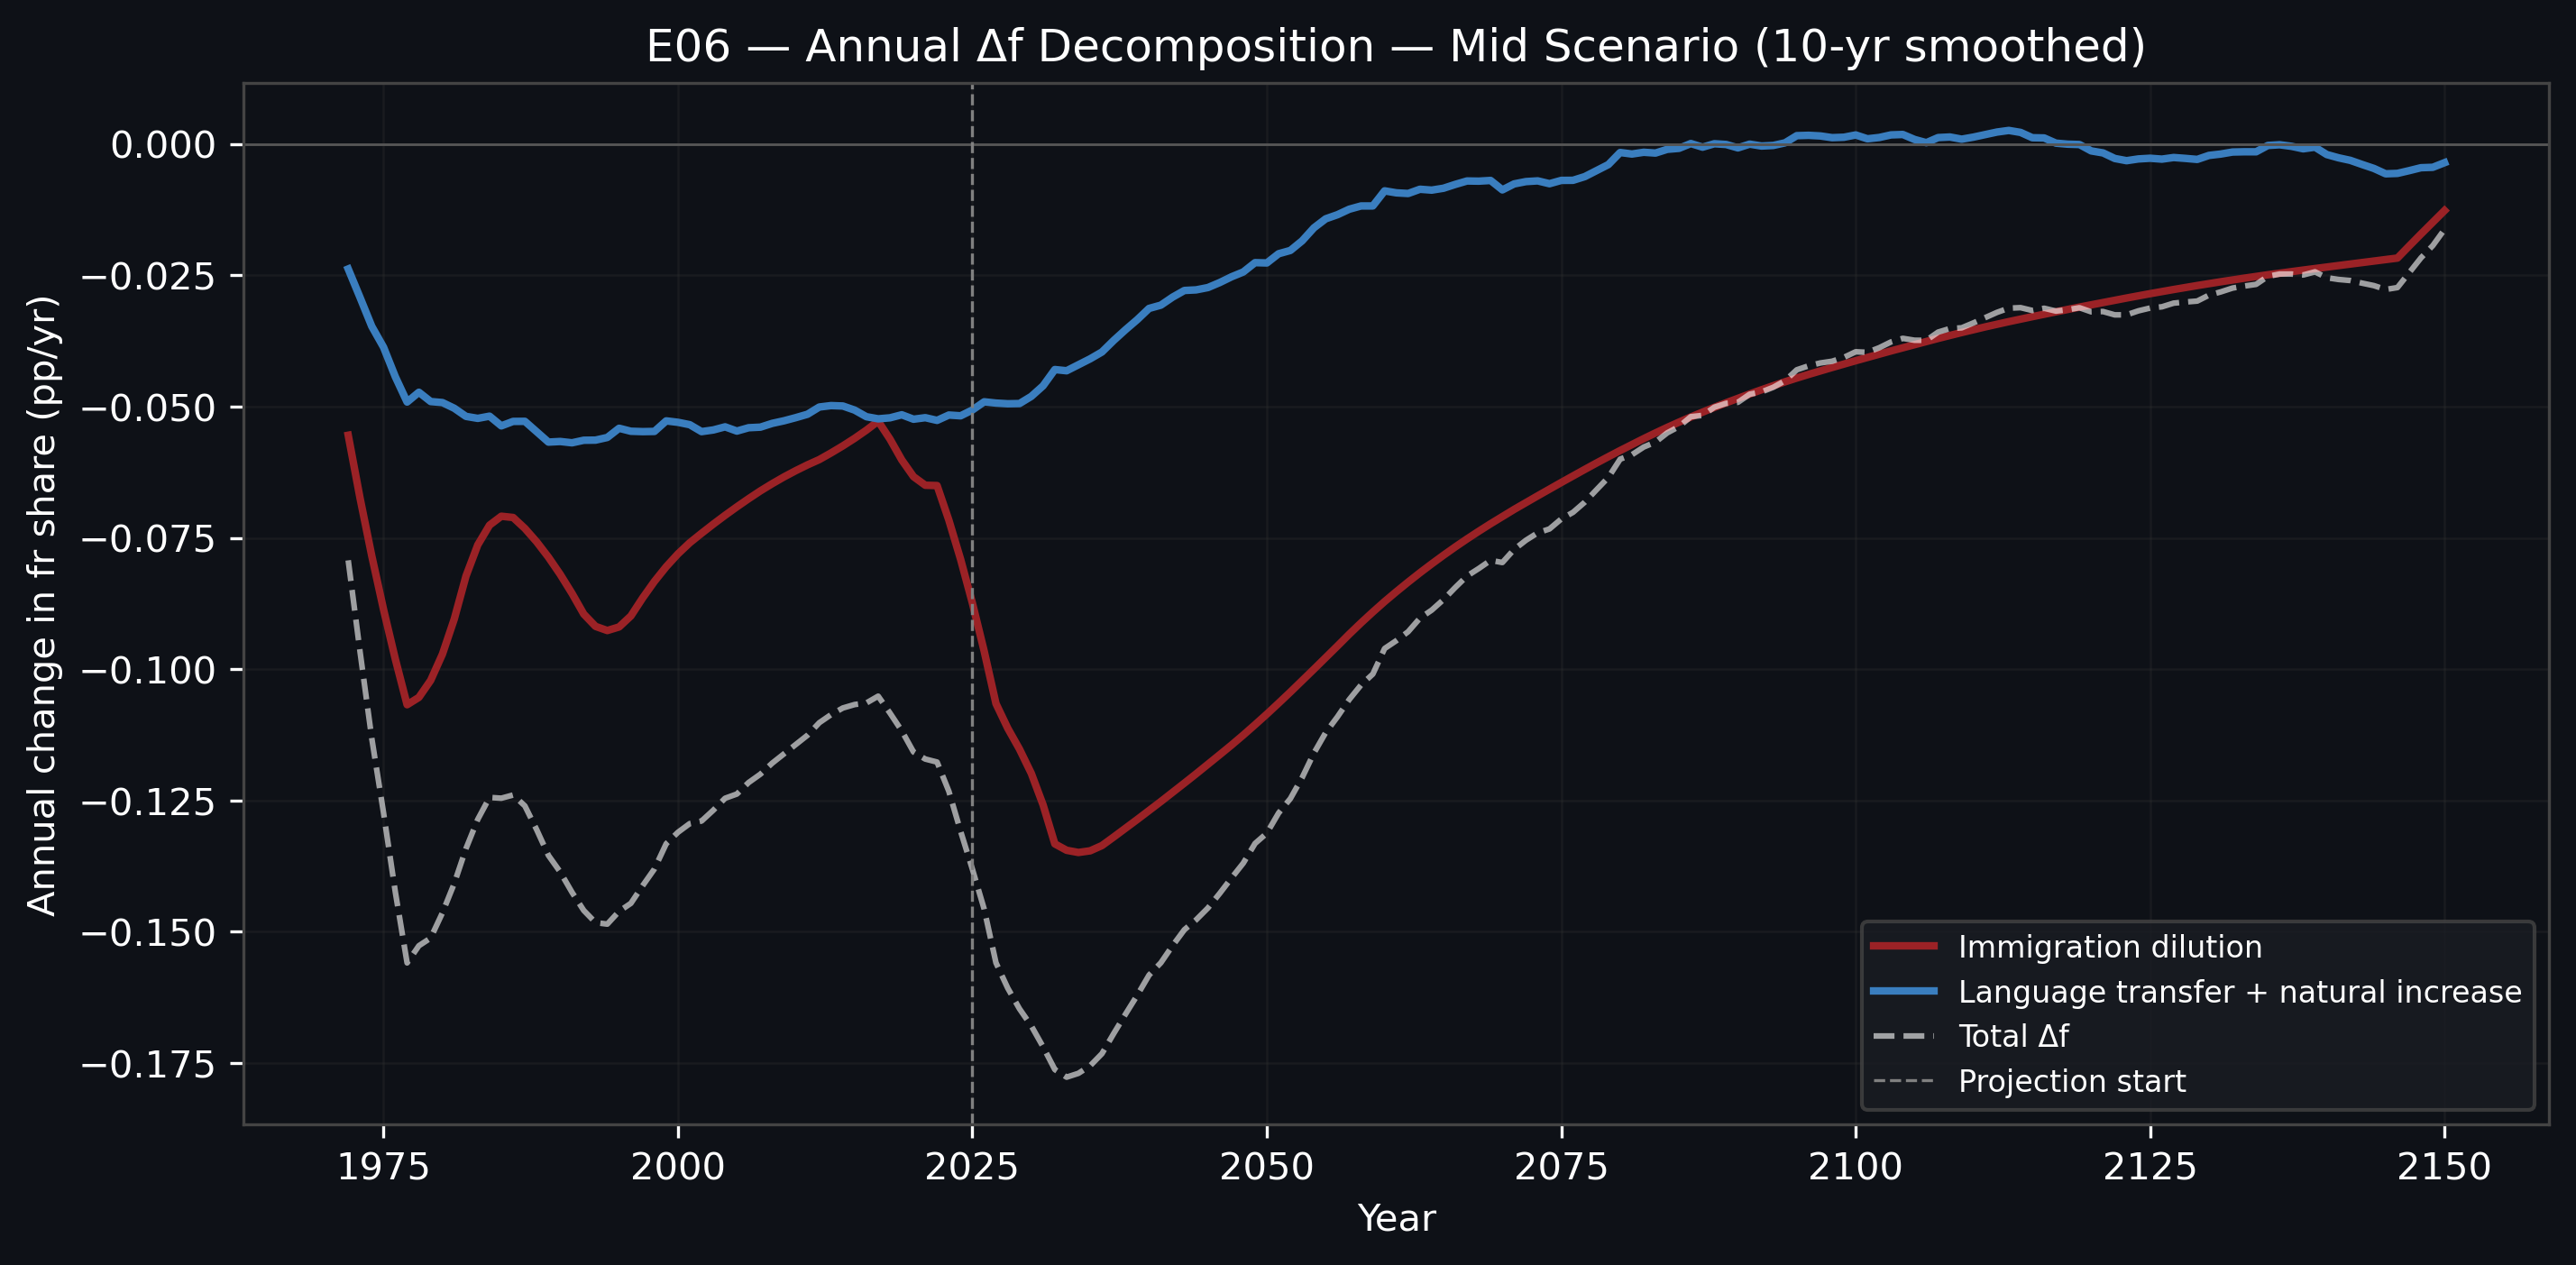
\includegraphics[width=\linewidth]{plots/E06_delta_f_decomposition_mid.png}
  \caption{Annual change in national francophone share decomposed into
           immigration dilution (red) and language transfer plus natural
           increase (blue), Mid scenario, 10-year smoothed.
           Immigration consistently dominates the decline.}
  \label{fig:decomp}
\end{figure}

Immigration dilution is the dominant and persistent force throughout.  The
language transfer contribution is negative but smaller, and diminishes after
2050 as the natural increase term (which is language-neutral in the model)
becomes negative across most provinces, partially offsetting assimilation
losses.  By 2100, the total annual change in share is less than 0.05
percentage points --- with immigration accounting for nearly all of it.

\begin{tcolorbox}[statbox]
\textbf{Policy implication.}  Because immigration dilution dominates, policies
that raise the francophone fraction of the immigrant intake have a far greater
impact on the trajectory than programmes targeting language transfer or
retention.  A 5 percentage point increase in the national immigrant
francophone share is worth more than eliminating French-to-English assimilation
in the ROC.
\end{tcolorbox}

\subsection{Finding 7 --- Stabilising the Share Would Require Doubling the
Immigrant Francophone Fraction}

Figure~\ref{fig:threshold} plots the francophone share of immigrants that
would be required each year to hold the national francophone share perfectly
flat (solid lines), alongside the actual $f_{\text{imm}}$ delivered in each
scenario (dashed lines).

\begin{figure}[H]
  \centering
  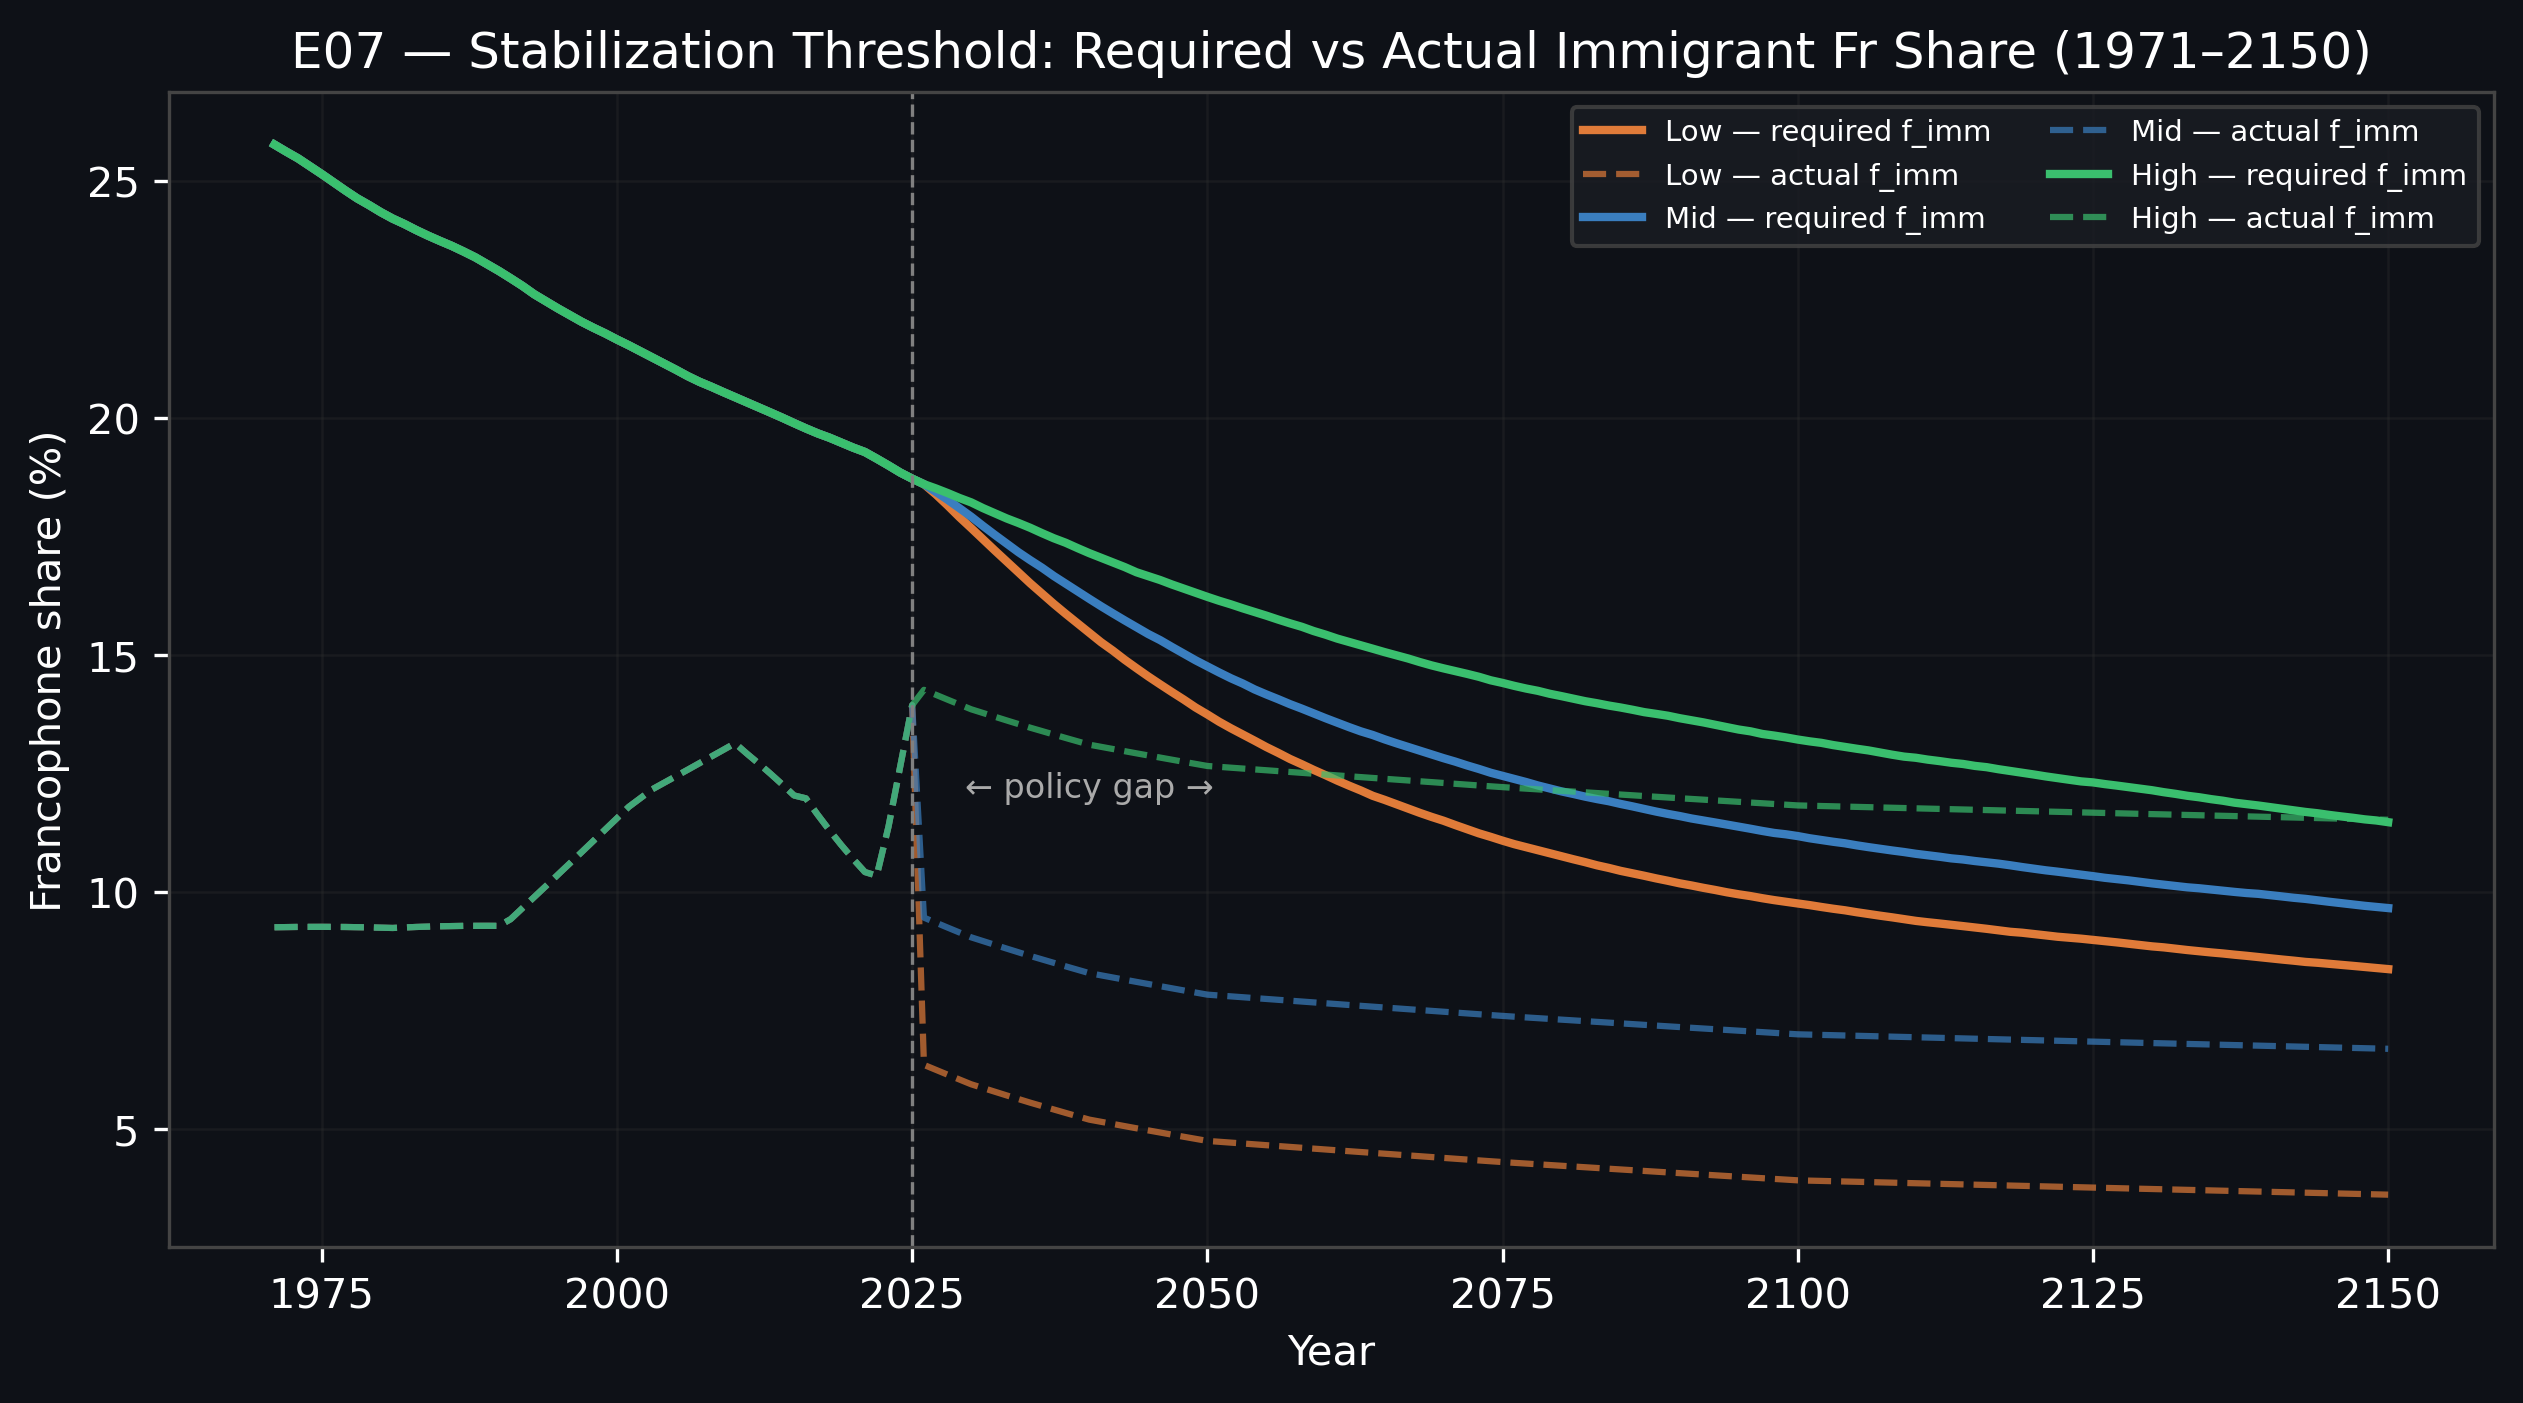
\includegraphics[width=\linewidth]{plots/E07_stabilization_threshold.png}
  \caption{Stabilisation threshold (solid): the francophone share of immigrants
           required to hold $f(t)$ constant, equal to $f(t)$ itself each year.
           Actual immigrant francophone share by scenario (dashed).
           The gap between solid and dashed is the policy shortfall.}
  \label{fig:threshold}
\end{figure}

In 2025 the stabilisation threshold stands at approximately 19\% --- meaning
19\% of all immigrants to Canada would need to be francophone to prevent any
decline.  The actual effective national $f_{\text{imm}}$ is approximately 6\%
(Low), 10\% (Mid), and 14\% (High), leaving a policy gap of 5--13 percentage
points.

As the share declines, the required threshold falls --- by 2075 it is
approximately 12\% under the Mid scenario --- and the High scenario comes
closest to closing it.  Even so, no scenario closes the gap within the
projection window.


% ═════════════════════════════════════════════════════════════════════════════
\section{Conclusions \& Strategic Implications}
% ═════════════════════════════════════════════════════════════════════════════

\begin{tcolorbox}[keybox, title=Summary of Conclusions]
\begin{enumerate}[leftmargin=1.2em]
  \item Francophone share decline is structural and cannot be reversed under
        any near-term realistic policy trajectory.
  \item Composition of immigration matters more than volume.
  \item The decline decelerates and does not produce demographic extinction.
  \item Quebec's position is resilient; the ROC is the existential front.
  \item The absolute francophone population grows, shifting the framing from
        survival to influence and institutional capacity.
\end{enumerate}
\end{tcolorbox}

\bigskip

\textbf{Composition, not volume, is the primary policy lever.}
The simulation demonstrates clearly that increasing immigration volumes without
raising the francophone share of arrivals worsens the outcome for French.
The Low scenario uses 10\% higher volumes than the Mid scenario yet produces
the worst results --- because the composition disadvantage compounds the volume.
Policy interventions aimed at increasing the francophone fraction of the intake
(recruitment in francophone Africa, QC selection regime continuity, ROC
francophone stream expansion) have a larger impact per dollar than equivalent
investments in post-arrival language retention.

\textbf{Quebec is not the concern; the ROC is.}
All scenarios project Quebec maintaining a francophone supermajority above 65\%
for the full projection period.  Bill 101, Quebec's selection powers, and the
extremely low out-migration of Quebec francophones together provide robust
demographic protection.  The crisis --- if there is one --- is in New
Brunswick and the rest of francophone Canada outside Quebec.  The ROC
francophone share is projected to halve from $\approx$5\% to $\approx$3--4\%
by 2150 even under the Mid scenario, driven simultaneously by dilution and
English assimilation.

\textbf{Absolute growth reframes the institutional challenge.}
The francophone population will grow from 7.5 million to 12--13 million by
2150.  This is not a community in numerical decline.  The challenge is one of
relative political weight, institutional funding formulas, and cultural
influence in a country that is growing faster still.  Policies calibrated to a
narrative of community survival may be less useful than policies calibrated to
maintaining institutional capacity for a growing population whose share of
national life is declining.

\textbf{Time matters.}  The plateau mechanism means that the window to
influence outcomes is concentrated in the near term.  The gap between the
current share and the immigrant fraction is widest now; each decade of
underperformance on francophone immigration targets locks in a lower
equilibrium.  Conversely, sustained ambition in the near term has compounding
benefits as the gap narrows and the system naturally stabilises at a higher
floor.

\bigskip
\begin{tcolorbox}[statbox]
\textbf{Model limitations.}  The simulation does not model age structure,
fertility differences by language group, socio-economic sorting, or policy
feedback loops.  All post-2025 inputs are projections, not forecasts.  The
model is a tool for understanding mechanisms and comparing scenarios, not for
producing point predictions of future demographic outcomes.
\end{tcolorbox}

\end{document}
